%==============================================================================
% tento soubor pouzijte jako zaklad
% this file should be used as a base for the thesis
% Autoři / Authors: 2008 Michal Bidlo, 2016 Jaroslav Dytrych
% Kontakt pro dotazy a připomínky: dytrych@fit.vutbr.cz
% Contact for questions and comments: dytrych@fit.vutbr.cz
%==============================================================================
% kodovani: UTF-8 (zmena prikazem iconv, recode nebo cstocs)
% encoding: UTF-8 (you can change it by command iconv, recode or cstocs)
%------------------------------------------------------------------------------
% zpracování / processing: make, make pdf, make clean
%==============================================================================
% Soubory, které je nutné upravit: / Files which have to be edited:
%   projekt-20-literatura-bibliography.bib - literatura / bibliography
%   projekt-01-kapitoly-chapters.tex - obsah práce / the thesis content
%   projekt-30-prilohy-appendices.tex - přílohy / appendices
%==============================================================================
%\documentclass[czech]{fitthesis} % bez zadání - pro začátek práce, aby nebyl problém s překladem
%\documentclass[english]{fitthesis} % without assignment - for the work start to avoid compilation problem
\documentclass[zadani]{fitthesis} % odevzdani do wisu - odkazy jsou barevné
%\documentclass[english,zadani]{fitthesis} % for submission to the IS FIT - links are color
%\documentclass[zadani,print]{fitthesis} % pro tisk - odkazy jsou černé
%\documentclass[zadani,cprint]{fitthesis} % pro barevný tisk - odkazy jsou černé, znak VUT barevný
%\documentclass[english,zadani,print]{fitthesis} % for the color print - links are black
%\documentclass[english,zadani,cprint]{fitthesis} % for the print - links are black, logo is color
% * Je-li práce psaná v anglickém jazyce, je zapotřebí u třídy použít 
%   parametr english následovně:
%   If thesis is written in english, it is necessary to use 
%   parameter english as follows:
%      \documentclass[english]{fitthesis}
% * Je-li práce psaná ve slovenském jazyce, je zapotřebí u třídy použít 
%   parametr slovak následovně:
%   If the work is written in the Slovak language, it is necessary 
%   to use parameter slovak as follows:
%      \documentclass[slovak]{fitthesis}
% * Je-li práce psaná v anglickém jazyce se slovenským abstraktem apod., 
%   je zapotřebí u třídy použít parametry english a enslovak následovně:
%   If the work is written in English with the Slovak abstract, etc., 
%   it is necessary to use parameters english and enslovak as follows:
%      \documentclass[english,enslovak]{fitthesis}

% Základní balíčky jsou dole v souboru šablony fitthesis.cls
% Basic packages are at the bottom of template file fitthesis.cls
% zde můžeme vložit vlastní balíčky / you can place own packages here

% Kompilace po částech (rychlejší, ale v náhledu nemusí být vše aktuální)
% Compilation piecewise (faster, but not all parts in preview will be up-to-date)
% \usepackage{subfiles}

% Nastavení cesty k obrázkům
% Setting of a path to the pictures
%\graphicspath{{obrazky-figures/}{./obrazky-figures/}}
%\graphicspath{{obrazky-figures/}{../obrazky-figures/}}

%---rm---------------
\renewcommand{\rmdefault}{lmr}%zavede Latin Modern Roman jako rm / set Latin Modern Roman as rm
%---sf---------------
\renewcommand{\sfdefault}{qhv}%zavede TeX Gyre Heros jako sf
%---tt------------
\renewcommand{\ttdefault}{lmtt}% zavede Latin Modern tt jako tt

% vypne funkci šablony, která automaticky nahrazuje uvozovky,
% aby nebyly prováděny nevhodné náhrady v popisech API apod.
% disables function of the template which replaces quotation marks
% to avoid unnecessary replacements in the API descriptions etc.
\csdoublequotesoff

% =======================================================================
% balíček "hyperref" vytváří klikací odkazy v pdf, pokud tedy použijeme pdflatex
% problém je, že balíček hyperref musí být uveden jako poslední, takže nemůže
% být v šabloně
% "hyperref" package create clickable links in pdf if you are using pdflatex.
% Problem is that this package have to be introduced as the last one so it 
% can not be placed in the template file.
\ifWis
\ifx\pdfoutput\undefined % nejedeme pod pdflatexem / we are not using pdflatex
\else
  \usepackage{color}
  \usepackage[unicode,colorlinks,hyperindex,plainpages=false,pdftex]{hyperref}
  \definecolor{links}{rgb}{0.4,0.5,0}
  \definecolor{anchors}{rgb}{1,0,0}
  \def\AnchorColor{anchors}
  \def\LinkColor{links}
  \def\pdfBorderAttrs{/Border [0 0 0] }  % bez okrajů kolem odkazů / without margins around links
  \pdfcompresslevel=9
\fi
\else % pro tisk budou odkazy, na které se dá klikat, černé / for the print clickable links will be black
\ifx\pdfoutput\undefined % nejedeme pod pdflatexem / we are not using pdflatex
\else
  \usepackage{color}
  \usepackage[unicode,colorlinks,hyperindex,plainpages=false,pdftex,urlcolor=black,linkcolor=black,citecolor=black]{hyperref}
  \definecolor{links}{rgb}{0,0,0}
  \definecolor{anchors}{rgb}{0,0,0}
  \def\AnchorColor{anchors}
  \def\LinkColor{links}
  \def\pdfBorderAttrs{/Border [0 0 0] } % bez okrajů kolem odkazů / without margins around links
  \pdfcompresslevel=9
\fi
\fi
% Řešení problému, kdy klikací odkazy na obrázky vedou za obrázek
% This solves the problems with links which leads after the picture
\usepackage[all]{hypcap}

% Informace o práci/projektu / Information about the thesis
%---------------------------------------------------------------------------
\projectinfo{
  %Prace / Thesis
  project={BP},            %typ práce BP/SP/DP/DR  / thesis type (SP = term project)
  year={2018},             % rok odevzdání / year of submission
  date=\today,             % datum odevzdání / submission date
  %Nazev prace / thesis title
  title.cs={Algoritmy pro automatický ořez fotografií},  % název práce v češtině či slovenštině (dle zadání) / thesis title in czech language (according to assignment)
  title.en={Algorithms for Automatic Image Cropping}, % název práce v angličtině / thesis title in english
  %title.length={14.5cm}, % nastavení délky bloku s titulkem pro úpravu zalomení řádku (lze definovat zde nebo níže) / setting the length of a block with a thesis title for adjusting a line break (can be defined here or below)
  %Autor / Author
  author.name={Vít},   % jméno autora / author name
  author.surname={Ambrož},   % příjmení autora / author surname 
  %author.title.p={Bc.}, % titul před jménem (nepovinné) / title before the name (optional)
  %author.title.a={Ph.D.}, % titul za jménem (nepovinné) / title after the name (optional)
  %Ustav / Department
  department={UPGM}, % doplňte příslušnou zkratku dle ústavu na zadání: UPSY/UIFS/UITS/UPGM / fill in appropriate abbreviation of the department according to assignment: UPSY/UIFS/UITS/UPGM
  % Školitel / supervisor
  supervisor.name={Martin},   % jméno školitele / supervisor name 
  supervisor.surname={Čadík},   % příjmení školitele / supervisor surname
  supervisor.title.p={Doc. Ing.},   %titul před jménem (nepovinné) / title before the name (optional)
  supervisor.title.a={Ph.D.},    %titul za jménem (nepovinné) / title after the name (optional)
  % Klíčová slova / keywords
  keywords.cs={algoritmy, ořez, automatický ořez, fotografie, C++, OpenCV}, % klíčová slova v českém či slovenském jazyce / keywords in czech or slovak language
  keywords.en={algorithms, cropping, automatic cropping, image, C++, OpenCV}, % klíčová slova v anglickém jazyce / keywords in english
  % Abstrakt / Abstract
  abstract.cs={Hlavním cílem této bakalářské práce je studium a implementace metod, které umožňují automatický ořez fotografií tak, aby výsledek ořezu byl použitelný z fotografického hlediska. V této práci jsou provedeny experimenty s třemi vybranými metodami a na jejich základě jsou diskutovány možné optimalizace. Jsou zde také popsány konkrétní vlastnosti jednotlivých algoritmů a provedeno zhodnocení výsledků automatického ořezu podle uživatelského testování.}, % abstrakt v českém či slovenském jazyce / abstract in czech or slovak language
  abstract.en={The main goal of this bachelor thesis is study and implementation of methods that can automatically crop images, so the result has good usability from a photographic view. In this thesis are made experiments with three methods and possible optimalizations are discussed. The properties of cropping algorithms are also described here and the evaluation of implemented algoritmhs is made according to user testing.}, % abstrakt v anglickém jazyce / abstract in english
  % Prohlášení (u anglicky psané práce anglicky, u slovensky psané práce slovensky) / Declaration (for thesis in english should be in english)
  declaration={Prohlašuji, že jsem tuto bakalářskou práci vypracoval samostatně pod vedením pana Doc. Ing. Martina Čadíka, Ph.D.
%Další informace mi poskytli...
Uvedl jsem všechny literární prameny a publikace, ze kterých jsem čerpal.},
  %declaration={Hereby I declare that this bachelor's thesis was prepared as an original author’s work under the supervision of Mr. X
% The supplementary information was provided by Mr. Y
% All the relevant information sources, which were used during preparation of this thesis, are properly cited and included in the list of references.},
  % Poděkování (nepovinné, nejlépe v jazyce práce) / Acknowledgement (optional, ideally in the language of the thesis)
  acknowledgment={Tímto bych velmi rád poděkoval Doc. Ing. Martinovi Čadíkovi, Ph.D. za poskytnutý čas, cenné rady a odborné vedení při řešení této práce.},
  %acknowledgment={Here it is possible to express thanks to the supervisor and to the people which provided professional help
%(external submitter, consultant, etc.).},
  % Rozšířený abstrakt (cca 3 normostrany) - lze definovat zde nebo níže / Extended abstract (approximately 3 standard pages) - can be defined here or below
  %extendedabstract={Do tohoto odstavce bude zapsán rozšířený výtah (abstrakt) práce v českém (slovenském) jazyce.},
  %faculty={FIT}, % FIT/FEKT/FSI/FA/FCH/FP/FAST/FAVU/USI/DEF
  faculty.cs={Fakulta informačních technologií}, % Fakulta v češtině - pro využití této položky výše zvolte fakultu DEF / Faculty in Czech - for use of this entry select DEF above
  faculty.en={Faculty of Information Technology}, % Fakulta v angličtině - pro využití této položky výše zvolte fakultu DEF / Faculty in English - for use of this entry select DEF above
  department.cs={Ústav matematiky}, % Ústav v češtině - pro využití této položky výše zvolte ústav DEF nebo jej zakomentujte / Department in Czech - for use of this entry select DEF above or comment it out
  department.en={Institute of Mathematics} % Ústav v angličtině - pro využití této položky výše zvolte ústav DEF nebo jej zakomentujte / Department in English - for use of this entry select DEF above or comment it out
}

% Rozšířený abstrakt (cca 3 normostrany) - lze definovat zde nebo výše / Extended abstract (approximately 3 standard pages) - can be defined here or above
%\extendedabstract{Do tohoto odstavce bude zapsán výtah (abstrakt) práce v českém (slovenském) jazyce.}

% nastavení délky bloku s titulkem pro úpravu zalomení řádku - lze definovat zde nebo výše / setting the length of a block with a thesis title for adjusting a line break - can be defined here or above
\titlelength{12.5cm}


% řeší první/poslední řádek odstavce na předchozí/následující stránce
% solves first/last row of the paragraph on the previous/next page
\clubpenalty=10000
\widowpenalty=10000

\begin{document}
  % Vysazeni titulnich stran / Typesetting of the title pages
  % ----------------------------------------------
  \maketitle
  % Obsah
  % ----------------------------------------------
  \setlength{\parskip}{0pt}

  {\hypersetup{hidelinks}\tableofcontents}
  
  % Seznam obrazku a tabulek (pokud prace obsahuje velke mnozstvi obrazku, tak se to hodi)
  % List of figures and list of tables (if the thesis contains a lot of pictures, it is good)
  \ifczech
    \renewcommand\listfigurename{Seznam obrázků}
  \fi
  \ifslovak
    \renewcommand\listfigurename{Zoznam obrázkov}
  \fi
  % \listoffigures
  
  \ifczech
    \renewcommand\listtablename{Seznam tabulek}
  \fi
  \ifslovak
    \renewcommand\listtablename{Zoznam tabuliek}
  \fi
  % \listoftables 

  \ifODSAZ
    \setlength{\parskip}{0.5\bigskipamount}
  \else
    \setlength{\parskip}{0pt}
  \fi

  % vynechani stranky v oboustrannem rezimu
  % Skip the page in the two-sided mode
  \iftwoside
    \cleardoublepage
  \fi

  % Text prace / Thesis text
  % ----------------------------------------------
  %=========================================================================
% (c) Michal Bidlo, Bohuslav Křena, 2008

%================== CHAPTER =====================%
\chapter{Úvod}
Ořez fotografie je v~současné době jedna z~nejpoužívanějších technik úpravy fotografií. Výběr optimálního rámečku ořezu z~fotografického hlediska je z~velké míry ovlivněn subjektivním pohledem na kompozici výsledné fotografie, dále je ovlivněn požadovanou šířkou a~výškou rámečku, a~také jejich vzájemným poměrem. Motivací pro vytvoření této práce je vytvoření efektivního řešení automatického ořezu pomocí existujících algoritmů. Automatický ořez fotografie by jistě mohl být prospěšný pro lidi, kteří mají malé zkušenosti s~vylepšením původní fotografie prostřednictvím ořezu a~chtěli by si své fotografie jednoduše a~rychle upravit. Za předpokladu, že vybrané metody ořezu umožní dosažení dobrého výsledku z~fotografického úhlu pohledu, by automatický ořez jistě ocenili i~zkušenější fotografové, například při ořezu velkého množství fotografií.

V~současné době existuje velké množství nástrojů, které umožňují manuální ořez fotografií. Tato práce se však věnuje problematice automatického ořezu fotografie, jehož cílem je dosáhnout nalezení optimálního rámečku na zadané fotografii tak, aby výsledek mohl být považován za použitelný z~fotografického hlediska. Hlavním kritériem pro určení míry kvality výsledného ořezu je zachování a~zdůraznění hlavních prvků, které jsou zachyceny na originální fotografii. Míra kvality výsledku automatického ořezu může být podrobněji hodnocena například podle základních vlastností kompozice fotografie. Cílem této práce je implementace algoritmů a~metod, které byly popsány v~odborných článcích, případně byly uvedeny v~rámci některé vědecké konference. Výsledky ořezů implementovaných metod budou v~této práci porovnány, budou uvedeny jejich výhody i~nevýhody, a~také budou v~rámci každé metody provedeny vlastní experimenty, na jejichž základě budou diskutovány možné optimalizace automatického ořezu.

Ve druhé kapitole této bakalářské práce je stručně popsána problematika obecného ořezu fotografií. Poté jsou zde uvedeny vybrané metody pro automatický ořez fotografií a~je vysvětlen jejich princip.

Ve třetí kapitole je popsán návrh implementace vybraných metod a~postup implementace v~případě obecného i~konkrétního hledání rámečku ořezu a~jeho případných optimalizací. Dále jsou zde uvedeny použité technologie, které byly použity pro implementaci.

Ve čtvrté kapitole je popsán návrh a~realizace testování, na jehož základě je provedeno porovnání a~zhodnocení výsledků automatického ořezu. Jsou zde uvedeny i~vlastní experimenty, kterými jsou demonstrovány různé vlastnosti vybraných algoritmů automatického ořezu.

V~poslední kapitole jsou shrnuty dosažené výsledky této práce a~diskutován možný budoucí vývoj.


%================== CHAPTER =====================%
\chapter{Metody pro automatický ořez fotografií}
\label{chapter:2}
V~této kapitole bude nejprve obecně popsána technika úpravy fotografií formou ořezu. Dále zde budou popsány jednotlivé metody, které jsem zvolil pro implementaci problematiky automatického ořezu fotografií. Také budou vysvětleny souvislosti, které jsou potřebné pro vytvoření a~pochopení jednotlivých metod.

%------------------ SECTION ---------------------%
\section{Ořez fotografie}
Ořez je jedna z~nejpoužívanějších a~nejdůležitějších technik úpravy fotografie, kterou je možné dosáhnout zlepšení estetické úrovně kvality oproti originální fotografii. Tohoto zlepšení lze dosáhnout tak, že je pozornost zaměřena na hlavní objekt či děj, který je zachycen na fotografii. Proto je důležité, aby z~originální fotografie byly odstraněny vedlejší či rušivé materiály, které ovlivňují lidské vnímání fotografie. 

Těmito materiály bývají často nevýrazné objekty v~pozadí, které nesouvisí s~hlavním objektem a~nejsou významné z~hlediska pozornosti. Nicméně právě tyto objekty či materiály mohou už na první pohled negativně ovlivnit celkové působení fotografie na člověka. Může se ovšem jednat i~o~objekty, které jsou v~popředí nebo na stejné úrovni jako je hlavní objekt. Těmi mohou být například objekty, které jsou na původní fotografii pouze z~části, což obvykle nemusí být záměrem. 

\paragraph{}
Prakticky je ořez fotografie proces, který jednak změní původní velikost fotografie, a~jednak také odstraní části, které nejsou ve výsledném rámečku ořezu zahrnuty. Kromě odstranění rušivých částí na původní fotografii, které byly výše zmíněny, zde ovšem vzniká riziko odstranění důležitých částí významných objektů. U~manuálního ořezu je toto riziko odstranění pochopitelně v~režii samotného fotografa a~někdy může být dokonce záměrem odstranit část hlavního prvku. 

U~automatického ořezu obrazu, kterému se tato práce věnuje, je ovšem možnost odstranění významných částí objektů velmi důležitým kritériem. Cílem je, aby k~odstranění hlavních částí docházelo co nejméně, nebo nejlépe vůbec. Příklad špatného ořezu, kde došlo ke zmíněnému odstranění důležité části, je znázorněn společně s~příkladem správného ořezu na obrázku \ref{obr:goodXbadCrop}.

\begin{figure}[H]
    \centering
    \begin{subfigure}{0.32\textwidth}
      \centering
      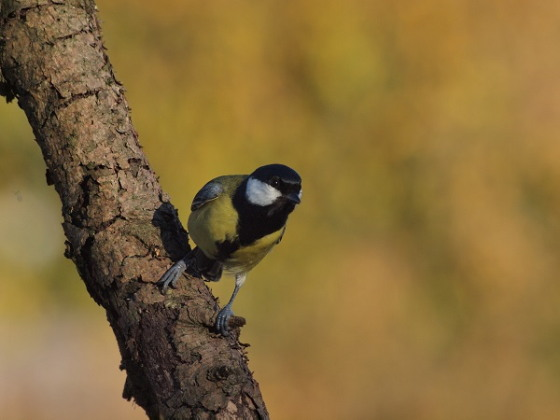
\includegraphics[scale=1.0]{obrazky/sykora.jpg}
      \caption{}
    \end{subfigure}
    \begin{subfigure}{0.32\textwidth}
      \centering
      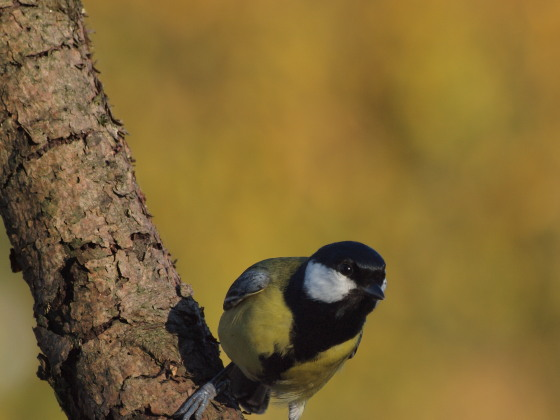
\includegraphics[scale=1.0]{obrazky/sykora-bad.jpg}
      \caption{}
    \end{subfigure}
    \begin{subfigure}{0.32\textwidth}
      \centering
      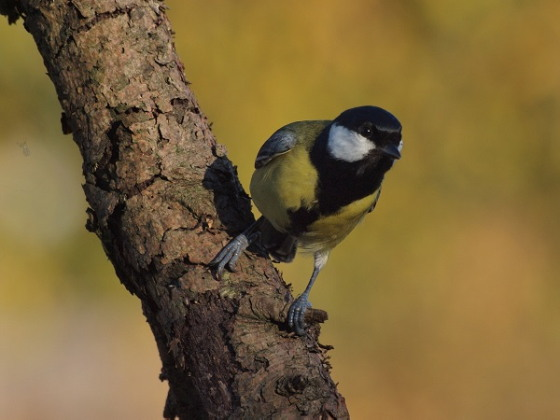
\includegraphics[scale=1.0]{obrazky/sykora-good.jpg}
      \caption{}
    \end{subfigure}
\caption{(a) Originální fotografie. (b) Příklad chybného ořezu, při kterém došlo k~odstranění důležité části hlavního objektu. (c) Příklad dobrého ořezu, kde byly zachovány všechny důležité části.}
\label{obr:goodXbadCrop}
\end{figure}

Důležitou vlastností fotografie je její kompozice \cite{Freeman2012}. Kompozicí je myšlen způsob uspořádání prvků či objektů na fotografii. Laikům by se mohlo zdát, že kompozice fotografie není příliš významná, opak je ale pravdou. Autor fotografie může totiž kompozicí mnohé sdělit. Fotograf by měl prvky na fotografii poskládat tak, aby působily na diváka harmonicky, anebo může jednoduše podpořit svůj záměr a~přitáhnout tak divákovu pozornost. Nicméně vnímání kompozice je z~velké míry subjektivní a~každý fotograf může preferovat jiná kompoziční řešení. Optimální kompozici nelze tedy přesně definovat. 

Široké možnosti a~experimenty s~kompozicí by určitě mohly být námětem pro samotnou diplomovou práci. Nicméně s~touto prací pochopitelně úzce souvisí, jelikož ořez je hlavní technikou pro vylepšení kompozice. Existuje spousta různých kompozičních pravidel. Pro ukázku bych zde rád uvedl alespoň dvě známá a~jednoduchá pravidla, které umožňují jistým způsobem vylepšit kompozici na základě umístění hlavních objektů na fotografii.

\paragraph{}
Prvním pravidlem je \emph{vlastnost zlatého řezu}. Ve své podstatě je zlatý řez konstantou, která má hodnotu přibližně $1,618$. Zlatý řez ve fotografii je považován za ideální proporci mezi délkami, které jsou určeny podle poměru $1:1,618$. Při využití této vlastnosti pro kompozici fotografie lze rámeček fotografie rozdělit v~horizontální i~vertikální rovině podle uvedeného poměru. Na základě tohoto rozdělení lze nalézt bod, který protnou přímky vedené rovnoběžně vertikální i~horizontální osou ve vzdálenosti podle uvedeného poměru. Je vhodné, aby podél přímek byly vedeny významné linie na fotografii a~v~jejich průsečíku byl umístěn hlavní objekt. Předpokládá se, že se lidské oko podvědomě zaměří na tento průsečík.

Další pravidlo kompozice, které se zlatým řezem souvisí, je \emph{pravidlo třetin}. Toto pravidlo vychází z~výše uvedených vlastností zlatého řezu. Poměr, kterým zlatý řez rozdělí rámeček fotografie, se dá považovat přibližně za dvě třetiny v~horizontální i~vertikální rovině. Hlavní objekt by podle tohoto pravidla měl být umístěn v~jednom ze 4 možných průsečíků. Jedná se tedy o~výrazné zjednodušení pravidla zlatého řezu, nicméně i~tak může často velmi pomoci ke zlepšení kompozice. Na obrázku \ref{obr:kompozice} je ukázka rozdílu mezi středovou kompozicí fotografie a~kompozicí při použití pravidla třetin.

V~praxi mohou být tyto pravidla kompozice výrazně ovlivněna počtem a~velikostí dalších objektů, které mají na výsledné fotografii být. Dále jsou ovlivněna i~tím, kolik prostoru má být kolem hlavního objektu ponecháno nebo je může ovlivnit například i~samotné pozadí fotografie. Nicméně se tyto základní pravidla považují za velmi užitečné a~jejich použitím lze obvykle dosáhnout slušných výsledků ořezu. 

\begin{figure}[H]
  \centering
  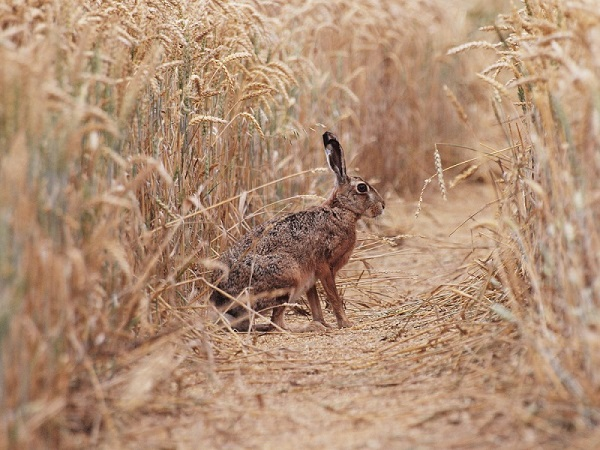
\includegraphics[scale=1.0]{obrazky/zajic-stred.jpg} \qquad
  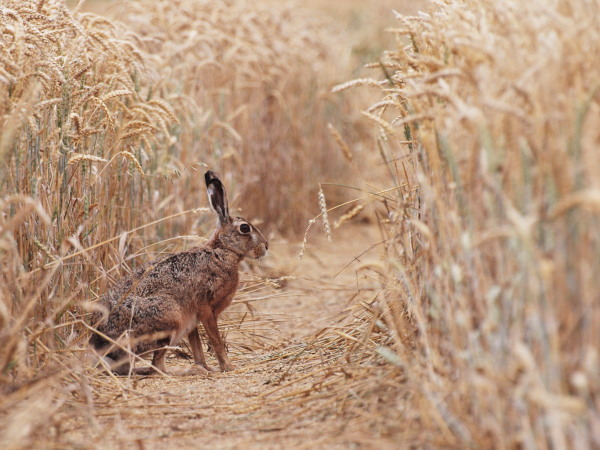
\includegraphics[scale=1.0]{obrazky/zajic-tretiny.jpg}
  \caption{Vlevo je příklad fotografie se středovou kompozicí. Vpravo je pro kompozici využito pravidlo třetin a~hlavní objekt je umístěn do levé dolní části.}
  \label{obr:kompozice}
\end{figure}


%------------------ SECTION ---------------------%
\section{Typy metod automatického ořezu} \label{section:typymetod}
Existuje mnoho kritérií a~technik, které se používají v~různých metodách automatického ořezu fotografií \cite{Yan2013}. Ze základního hlediska lze metody automatického ořezu rozdělit na dva obecné typy, které se zaměřují na odlišné faktory či vlastnosti.

\subsection{Attention-based metody} \label{section:attention-metody}
Prvním typem jsou \emph{metody založené na pozornosti(attention-based)}. Tyto metody se soustředí na detekování a~nalezení hlavních objektů nebo důležitých oblastí na fotografii. K~jejich nalezení potřebují nějakým způsobem získat reprezentaci míry významu jednotlivých částí fotografie. Většina těchto metod definuje vlastní algoritmy, podle kterých se vypočte oblast s~nejvyšší mírou pozornosti, a~kolem ní je umístěn rámeček ořezu.

Tyto metody většinou spolehlivě odstraní zbytečný a~rušivý obsah z~originální fotografie, a~zároveň ponechají hlavní objekt ve výsledném rámečku. Nicméně žádným způsobem neřeší jeho kompozici a~umístění ve výsledném ořezu. Výsledek pak nemusí na diváka působit harmonicky.

\paragraph{}
Stanovení míry pozornosti částí fotografie lze dosáhnout různými technikami. Může se jednat o~velmi specifický případ detekce konkrétních objektů. Taková metoda automatického ořezu může být založena například na detekci obličejů \cite{Zhang2005}, kde část obsahující obličej bude mít vyšší míru pozornosti než ostatní části fotografie.

V~jiných případech tyto metody používají trochu obecnější reprezentaci pozornosti a~významu částí fotografie. Tento význam bývá často reprezentován pomocí tzv. \emph{saliency map} \cite{Achanta2009,Itti1998,Margolin2013,Stentiford2007}, která může být vypočtena pomocí různých algoritmů. Algoritmus pro výběr optimálního rámečku ořezu pak může být založen například na nejvyšší průměrné míře pozornosti jednotlivých pixelů \cite{Stentiford2007} nebo na poměru míry významu rámečku ořezu vůči celkové hodnotě míry významu originální fotografie \cite{Suh2003}.


\subsection{Aesthetics-based metody} \label{section:aesthetics-metody}
Druhým obecným typem metod automatického ořezu obrazu jsou \emph{metody založené na estetice(aesthetics-based)}. Tyto metody kladou důraz na vlastnosti související s~kompozicí fotografie. Jejich cílem je dosáhnout vhodného rozložení objektů a~zajištění atraktivity fotografie pro diváka. Jejich nevýhodou může být v~některých případech situace, kdy nedojde k~oříznutí nechtěného a~rušivého obsahu na originální fotografii.

Tyto metody určitým způsobem posuzují vlastnosti kompozice tak, aby mohly na jejich základě vybrat rámeček ořezu a~vylepšit tak estetickou kvalitu fotografie \cite{Luo2007,Tang2013}. Vlastnosti kompozice mohou být ručně definovány nebo může být případně vytvořen model, který je natrénován z~vhodné sady fotografií splňující konkrétní podmínky kompozice.

\paragraph{}
Metody automatického ořezu by pochopitelně bylo možné rozdělit podle množství jiných kritérií, nicméně výše uvedené směry jsou pravděpodobně nejobecnějším dělením. Oba typy vycházejí z~důležitých vlastností či cílů ořezu, kterými jsou zdůraznění hlavních objektů, odstranění rušivých elementů a~také vylepšení kompozice fotografie. Existují ale i~metody, které jsou v~podstatě kombinací výše uvedených typů \cite{Fang2014,Yan2013}. Právě tyto metody při kvalitativních porovnáních ořezů dosahují nejlepších výsledků.

V~rámci této práce jsem si zvolil a~implementoval dvě základní metody \cite{Stentiford2007,Suh2003}, které zastupují skupinu metod prvního typu uvedeného výše. Jinými slovy jsou založeny na pozornosti a~významu jednotlivých částí fotografie. Také jsem implementoval metodu automatického ořezu \cite{Fang2014}, která reprezentuje kombinaci obou typů. Tato metoda je novější a~robustnější, a~měla by dosahovat lepších výsledků ořezu. Vybrané metody budou podrobněji popsány v~následujících sekcích.

Důvodem, proč jsem si nevybral nejmodernější metody automatického ořezu, je skutečnost, že vybrané metody představují opravdový základ pro porozumění problematice. Navíc se spousta novějších metod částečně inspiruje vybranými metodami a~odkazuje se na ně. Implementace některých novějších metod by byla jistě zajímavá z~pohledu budoucího vývoje. 


%------------------ SECTION ---------------------%
\section{Attention Based Auto Image Cropping} \label{section:metoda1}
Tato metoda automatického ořezu obrazu \cite{Stentiford2007} se zaměřuje na výběr optimálního rámečku podle míry vizuální pozornosti jednotlivých částí na fotografii. Je postavena na předpokladu, že fotografie obsahují vizuálně významné oblasti, které jsou obklopeny částmi méně významného materiálu, například rušivým pozadím. Dále mohou být obklopeny částmi, které nesouvisí s~hlavním objektem, respektive důležitým dějem, který je na fotografii zachycen. 

Pro lidské oko vypadá mnohem lépe oříznutý obrázek, kde je zdůrazněn hlavní prvek a~je zde co nejméně dalších objektů či materiálů, které odtahují pozornost od hlavního objektu. Tato metoda automatického ořezu si tedy klade za cíl především zachovat hlavní prvky a~sdělení fotografie, které jsou charakterizovány vysokou mírou vizuální pozornosti. Tento algoritmus nebere v~potaz kompozici fotografie a~tedy výběr nejlepšího možného ořezu nelze kompozičně nijak hodnotit.

\subsection{Saliency map} 
Aby bylo možné získat optimální rámeček, který bude výstupem automatického ořezu v~této metodě, je třeba nejprve vytvořit tzv. \emph{saliency map}. Tato \emph{saliency map}, jak ji zde budu označovat, představuje význam jednotlivých částí, respektive samotných pixelů, na originální fotografii. V~této metodě je popsán obecný algoritmus pro vytvoření \emph{saliency} map, která se pro výpočet používá. Její příklad, vytvořený pro danou fotografii, je zobrazen na obrázku \ref{obr:StentSalMap}. Čím je část fotografie důležitější z~hlediska pozornosti, tím vyšší hodnoty bude na této \emph{saliency map} mít. Části, které jsou významově důležité, jsou zde tedy reprezentovány světlejšími barvami.

Oblast na originální fotografii, která je podobná většině ostatních oblastí, bude pravděpodobně součástí některého většího celku, například šumu v~pozadí. Takovéto oblasti by měly dosáhnout malé významové hodnoty. Naopak hrany a~okraje větších objektů nebo některé různě barevné prvky budou pravděpodobně dosahovat vyšších významových hodnot. 

\begin{figure}[H]
    \centering
    \begin{subfigure}{0.5\textwidth}
      \centering
      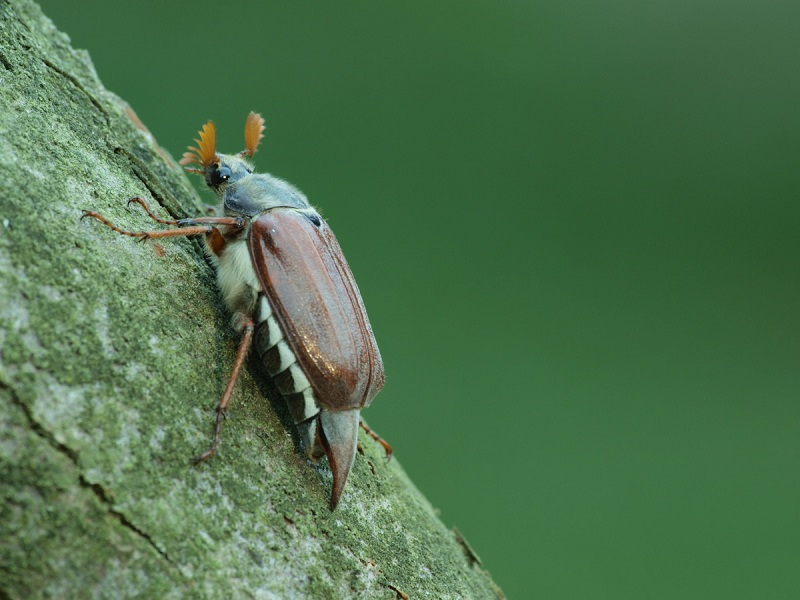
\includegraphics[scale=1.0]{obrazky/ORIGbrouk.JPG}
      \caption{Originální fotografie}
      \label{obr:original}
    \end{subfigure}
    \begin{subfigure}{.49\textwidth}
      \centering
      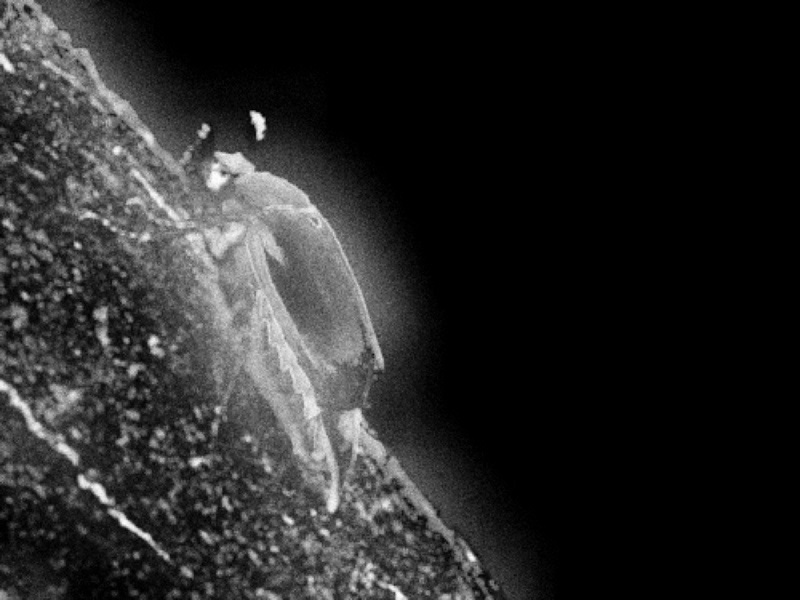
\includegraphics[scale=1.0]{obrazky/StentifordSMbrouk.jpg}
      \caption{Saliency map}
      \label{obr:saliency}
    \end{subfigure}
    \caption{Originální fotografie a~její \emph{saliency map} \cite{Stentiford2007}}
\label{obr:StentSalMap}
\end{figure}

V~této metodě vytváření \emph{saliency map} jsou významné části fotografie detekovány procesem, který vzájemně porovnává malé oblasti na fotografii. Oblastí se zde rozumí skupina několika pixelů, které jsou v~blízkém okolí aktuální pixelu, pro který se provádí výpočet. Tento pixel označme jako $x$ a~jeho horizontální a~vertikální souřadnici $x_1$ a~$x_2$. Jeho funkční hodnota je označena jako $F(x)$ a~představuje barevné složky $a_1, a_2, a_3$ tohoto pixelu. Formální zápis pixelu je zobrazen na rovnicích \ref{equation:2.1}.

\begin{equation} \label{equation:2.1}
x = (x_1, x_2), \quad F(x) = (a_1, a_2, a_3)
\end{equation}

Ke každému pixelu je vytvořena vlastní oblast, která je součástí jeho nejbližšího okolí $N$. Maximální možná vzdálenost pixelu $x_i^{\prime}$ patřícího do okolí $N$ od aktuálního pixelu $x_i$, nesmí být vyšší než vzdálenost definovaná parametrem $\epsilon_i$. Matematicky to lze zapsat například pomocí vztahu \ref{equation:2.2}.

\begin{equation} \label{equation:2.2}
\{ x^{\prime} \in N \Leftrightarrow \lvert x_i - x_i^{\prime} \rvert \leq \epsilon_i \quad \forall i~\}
\end{equation}

Oblast se skládá z~definovaného množství $m$ náhodně zvolených pixelů patřících do okolí $N$. Tuto oblast je možné označit jako $S_A$ a~definovat ji pomocí vztahu \ref{equation:2.3}.

\begin{equation} \label{equation:2.3}
S_A = \{ x_1^{\prime}, x_2^{\prime}, x_3^{\prime}, \dots, x_m^{\prime} \}
\end{equation}

\begin{figure}[H]
    \centering
    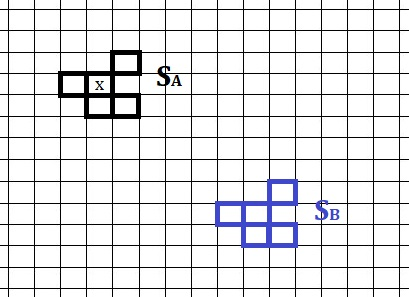
\includegraphics[scale=0.75]{obrazky/forks.jpg}  
    \caption{Grafické znázornění oblasti $S_A$, která je vytvořena kolem pixelu $x$. Zde je použito omezení okolí vzdáleností 2 od pixelu $x$. Poté je možné vytvořit oblast $S_B$ posunutím oblasti $S_A$.}
	\label{obr:forks}
\end{figure}

Pro každou oblast $S_A$ se provede porovnání s~daným množstvím dalších oblastí $S_B$, které mají stejné uspořádání, ale nachází se v~jiné části fotografie. Prakticky to znamená, že pro vytvoření oblasti $S_B$ je provedeno posunutí původní oblasti $S_A$. Příklad oblastí $S_A$ a~$S_B$ je graficky znázorněn na obrázku \ref{obr:forks}. Posunutí může probíhat libovolným horizontálním a~vertikálním směrem, pokud to umožňují hranice fotografie. Například pixel, respektive pro něj vytvořenou oblast $S_A$, která se nachází v~levém horním rohu rámečku, bude možné posunout pouze vertikálně dolů a~horizontálně doprava. Oblast $S_B$ je formálně zapsána vztahem \ref{equation:2.4}.

\begin{equation} \label{equation:2.4}
S_B = \{ y_1, y_2, y_3, \dots, y_m \}
\quad and \quad x_i - y_i = \delta_j
\end{equation}

Porovnání oblastí se provádí na základě barevných hodnot pixelů v~oblastech. Je zde třeba definovat prahovou hodnotu $\tau_j$ pro maximální hranici mezi rozdíly barev jednotlivých pixelů. Pokud některý z~pixelů z~první oblasti přesáhne definovanou prahovou hodnotu rozdílu barev oproti příslušnému pixelu z~druhé oblasti, je první oblast považována za rozdílnou z~hlediska pozornosti. Dochází k~navýšení míry vizuální pozornosti pro aktuální pixel $x$, pro který byla oblast vytvořena. Oblast $S_A$ neodpovídá oblasti $S_B$, pokud nastane situace určená vztahem \ref{equation:2.5}.

\begin{equation} \label{equation:2.5}
\lvert F_j(x_i) - F_j(y_i) \rvert \geq \tau_j \qquad for\; any\; i,j
\end{equation}

Pokud je vygenerováno dostatečné množství oblastí, se kterými se bude aktuální oblast porovnávat, budou se postupně zvyšovat míry pozornosti pro pixely vizuálně významné oblasti. Pro méně výrazné a~důležité oblasti se tato míra zvyšovat pochopitelně příliš nebude. V~praxi to může být jednoduše reprezentováno například vytvořením \emph{saliency map} pouze s~jedním kanálem barev. Černá barva tedy představuje oblasti s~nejmenší mírou vizuální pozornosti a~naopak bílá představuje hodnoty s~nejvyšší mírou pozornosti tak, jak je tomu na obrázku \ref{obr:saliency}.

Výsledná \emph{saliency map} může být ovlivněna několika parametry či faktory, kterými jsou například prahová hodnota $\tau_j$, počet pixelů v~oblastech $S_A$ a~$S_B$ nebo způsob výpočtu barevných komponent pixelu. Tyto parametry mohou mít pro fotografie různých typů odlišné hodnoty pro získání dobrého výsledku, a~proto jsem s~nimi vyzkoušel několik experimentů. Experimenty s~výše uvedenými parametry budou podrobněji popsány v~rámci sekce \ref{sekce:expmetody}.

\subsection{Výběr nejlepšího rámečku}
Optimální rámeček je vybrán podle barevných hodnot získaných ze \emph{saliency map}. Reprezentace míry pozornosti je zde postavena na základě výzkumu Shilstona a~Stentiforda \cite{Shilston2006}, kde je maximální míra pozornosti použita pro zaměření hlavního prvku fotografie. Míra pozornosti $M_I$ konkrétního rámečku je definována podle rovnice \ref{equation:2.6}. 

\begin{equation} \label{equation:2.6}
M_I = \sum_{x \in I} V(x)
\end{equation}

Míra vizuální pozornosti konkrétního rámečku $I$ je součet míry pozornosti jednotlivých pixelů, které do rámečku $I$ patří. Míry pozornosti pixelů $V(x)$ jsou reprezentovány hodnotami ze~\emph{saliency map}.

Definice nejlepšího rámečku $W_I$ pro automatický ořez je popsána rovnicí \ref{equation:2.7}. Jedná se tedy o~maximalizaci funkce, která popisuje průměrnou míru pozornosti pro jeden pixel v~daném rámečku $W$ z~množiny všech rámečků $I$.

\begin{equation} \label{equation:2.7}
W_I = \arg\max_{W \in I} \sum_{x \in W} V(x)/\lVert{W}\rVert
\end{equation}

Principy vytvořených funkcí, pro které byl použit tento algoritmus výběru rámečku, budou podrobněji uvedeny v~sekci \ref{sekce:navrh_metody}. Nejzákladnějším způsobem může být optimální rámeček hledán použitím výpočtů hrubé síly, což prakticky znamená, že budou rámečky vytvářeny na všech pozicích a~počítány pro všechny možné velikosti. Jelikož je tento způsob časově neefektivní, bude vhodné se věnovat možnostem, jak jej zlepšit.

Na obrázku \ref{obr:stentifordCrop} jsou zobrazeny fotografie, pro které tato metoda s~použitím uvedené \emph{saliency map} proběhla ze základního fotografického hlediska dobře. Výsledné ořezy byly provedeny pro zmenšení na 2/3 původní velikosti fotografie se zachováním poměru šířky a~výšky.

\begin{figure}[H]
    \centering
    \begin{subfigure}{0.32\textwidth}
      \centering
      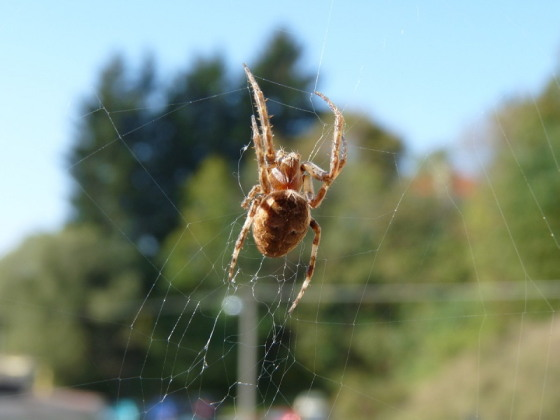
\includegraphics[scale=1.0]{obrazky/ORIGpavouk.JPG}
    \end{subfigure}
    \begin{subfigure}{.32\textwidth}
      \centering
      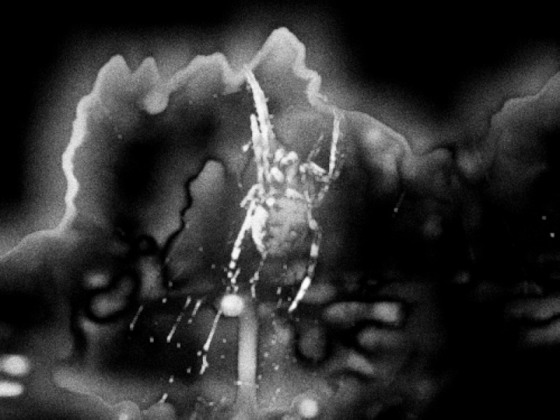
\includegraphics[scale=1.0]{obrazky/StentifordSMpavouk.jpg}
    \end{subfigure}
    \begin{subfigure}{.32\textwidth}
      \centering
      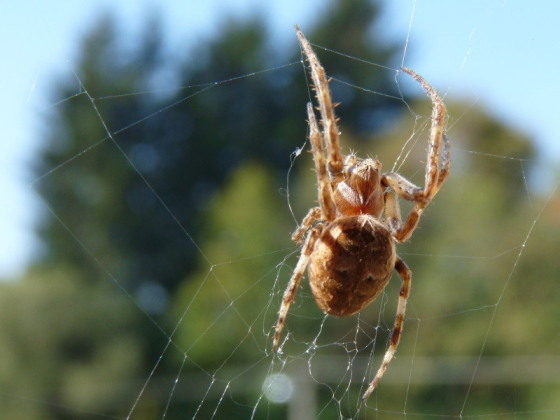
\includegraphics[scale=1.0]{obrazky/cropStentifordpavouk.jpg}
    \end{subfigure}
    \vspace{2pt}
    
    \begin{subfigure}{0.32\textwidth}
      \centering
      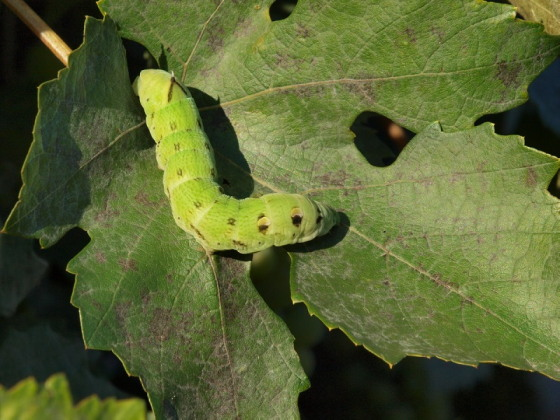
\includegraphics[scale=1.0]{obrazky/ORIGhousenka.JPG}
    \end{subfigure}
    \begin{subfigure}{.32\textwidth}
      \centering
      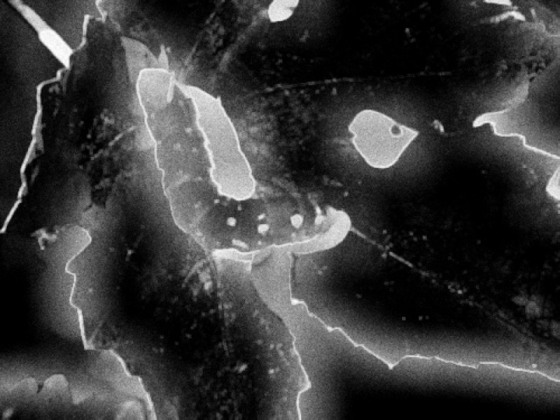
\includegraphics[scale=1.0]{obrazky/StentifordSMhousenka.jpg}
    \end{subfigure}
    \begin{subfigure}{.32\textwidth}
      \centering
      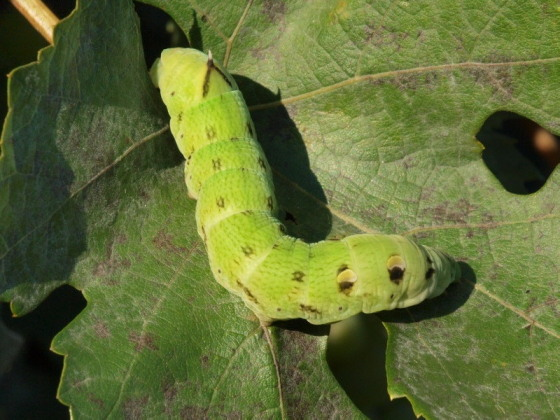
\includegraphics[scale=1.0]{obrazky/cropStentifordhousenka.jpg}
    \end{subfigure}
    \vspace{2pt}
    
    \begin{subfigure}{0.32\textwidth}
      \centering
      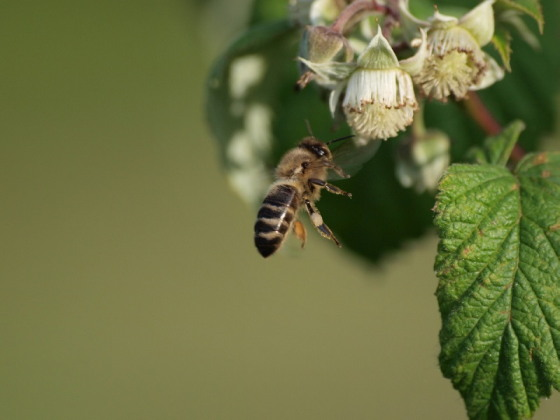
\includegraphics[scale=1.0]{obrazky/ORIGvcela.JPG}
      \caption{}
    \end{subfigure}
    \begin{subfigure}{.32\textwidth}
      \centering
      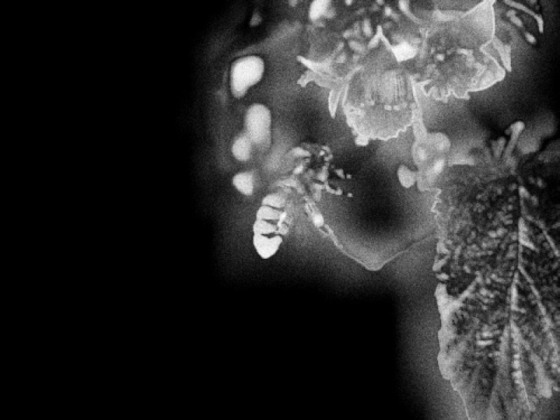
\includegraphics[scale=1.0]{obrazky/StentifordSMvcela.jpg}
      \caption{}
    \end{subfigure}
    \begin{subfigure}{.32\textwidth}
      \centering
      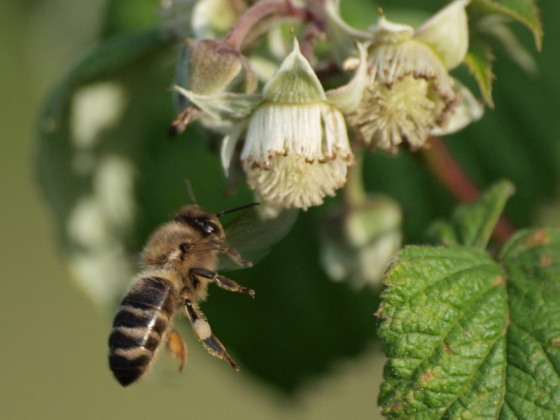
\includegraphics[scale=1.0]{obrazky/cropStentifordvcela.jpg}
      \caption{}
    \end{subfigure}
    \vspace{2pt}
    
\caption{(a) Originální fotografie. (b) \emph{Saliency maps} vytvořené pro jednotlivé fotografie. (c) Automatický ořez \cite{Stentiford2007} původní fotografie se zachováním poměru velikosti šířky a~výšky rámečku (2/3 původní velikosti).}
\label{obr:stentifordCrop}
\end{figure}

\subsection{Problém definice velikosti rámečku ořezu}
S~výběrem nejlepšího rámečku souvisí i~problém definice velikosti jeho rozměrů a~právě zde přichází v~potaz nevýhoda tohoto algoritmu. Rovnice \ref{equation:2.2} jasně definuje, že optimální rámeček bude nalezen na základě nejvyšší průměrné míry pozornosti na jeden pixel rámečku. Problém spočívá v~tom, že tato metoda nelze použít obecně, jelikož by ve většině případů docházelo k~tomu, že by nejvyšší průměrná míra pozornosti byla nalezena pro velmi malý rámeček. Tato metoda by tak mohla v~extrémní situaci konvergovat až k~velikosti rámečku 1x1 pixel, byl by tedy zvolen pixel s~nejvyšší mírou pozornosti.

V~článku, který popisuje tuto metodu \cite{Stentiford2007}, byla provedena diskuze především pro hledání rámečku ořezu se zachováním původní poměru šířky a~výšky. Protože zůstává zachován původní poměr stran, tak je zde vytvořen parametr, který udává, kolikrát bude rámeček ořezu menší oproti původní fotografii. Tento parametr je zde označen jako \emph{faktor přiblížení(zoom factor)}. Pokud bude nastaven například na hodnotu $3.0$, tak šířka i~výška rámečku ořezu bude mít velikost $1/3$ původních velikostí. Pro lepší pochopení je použití \emph{faktoru přiblížení} znázorněno na obrázku \ref{obr:zoomFactors}.


\begin{figure}[H]
    \centering
    \begin{subfigure}{0.4\textwidth}
      \centering
      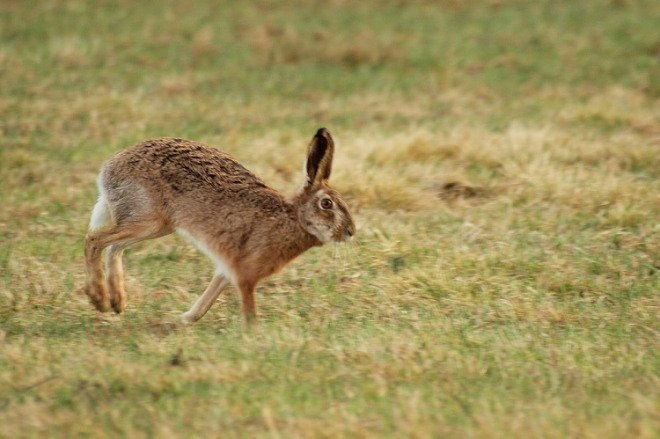
\includegraphics[scale=1.0]{obrazky/ORIGzajic6.jpg}
      \caption{Originální obrázek}
    \end{subfigure}
    \begin{subfigure}{0.4\textwidth}
      \centering
      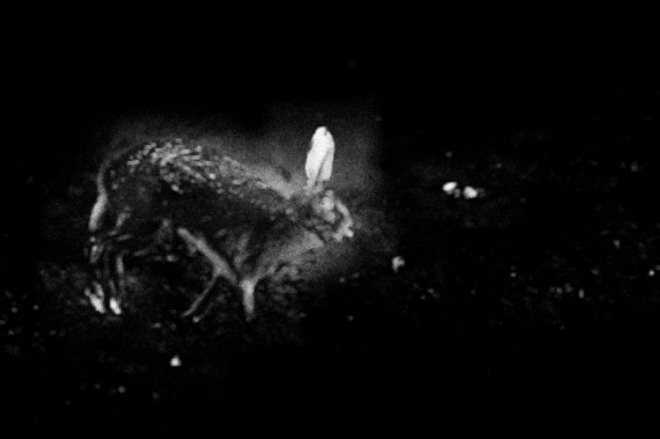
\includegraphics[scale=1.0]{obrazky/StentifordSMzajic6.jpg}
      \caption{Saliency map}
    \end{subfigure}
    \vspace{2pt}
    
    \begin{subfigure}{0.3\textwidth}
      \centering
      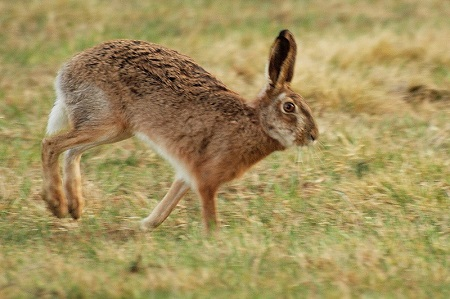
\includegraphics[width=35mm]{obrazky/cropStentiford1_5zajic6.jpg}
      \caption{$Zoom factor = 1.5$}
    \end{subfigure}
    \begin{subfigure}{0.3\textwidth}
      \centering
      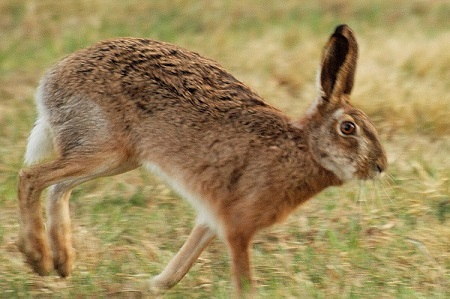
\includegraphics[width=35mm]{obrazky/cropStentiford2zajic6.jpg}
      \caption{$Zoom factor = 2.0$}
    \end{subfigure}
    \begin{subfigure}{0.3\textwidth}
      \centering
      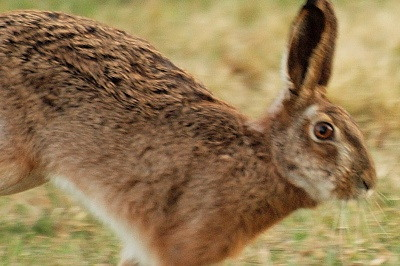
\includegraphics[width=35mm]{obrazky/cropStentiford3zajic6.jpg}
      \caption{$Zoom factor = 3.0$}
    \end{subfigure}
    \vspace{2pt}
    
    \begin{subfigure}{0.3\textwidth}
      \centering
      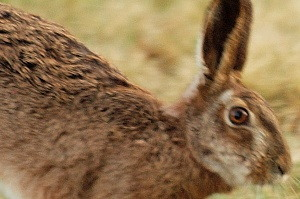
\includegraphics[width=25mm]{obrazky/cropStentiford4zajic6.jpg}
      \caption{$Zoom factor = 4.0$}
    \end{subfigure}
    \begin{subfigure}{0.3\textwidth}
      \centering
      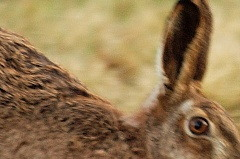
\includegraphics[width=25mm]{obrazky/cropStentiford5zajic6.jpg}
      \caption{$Zoom factor = 5.0$}
    \end{subfigure}
    \begin{subfigure}{0.3\textwidth}
      \centering
      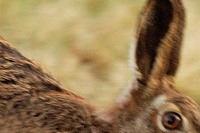
\includegraphics[width=25mm]{obrazky/cropStentiford6zajic6.jpg}
      \caption{$Zoom factor = 6.0$}
    \end{subfigure}
    
\caption{Ukázka ořezů fotografie se zachováním poměru stran a~se zvyšujícím se \emph{faktorem přiblížení(zoom factor)}. Je zřejmé, že pro tuto fotografii by tato metoda obecně konvergovala k~velmi malým velikostem rámečku, kde by byla nejvyšší průměrná míra pozornosti.}
\label{obr:zoomFactors}
\end{figure}

Tento algoritmus automatického ořezu je velmi vhodné použít v~případech, kdy je přesně stanovena šířka a~výška rámečku ořezu. Obecný postup pro nalezení rámečku ořezu, pokud nejsou zadány jeho rozměry, tato metoda přesně nedefinuje. Nicméně hledání rámečku lze provádět například postupným zvyšováním \emph{faktoru přiblížení} nebo případně snižováním velikosti šířky a~výšky rámečku. Zároveň je ale nezbytné definovat spodní omezení velikosti rámečku. Toto omezení by mělo zajistit, aby nedocházelo k~výběru extrémně malého rámečku. I~tak by byl pravděpodobně velmi často vybrán rámeček ořezu, který by velikostně odpovídal tomuto omezení, jelikož by jeho průměrná míra pozornosti byla nejvyšší.

Pokud by byla zadefinována velmi malá velikost rámečku oproti originální fotografii, mohlo by být praktické použít algoritmus ořezu rekurzivně. Výsledný rámeček ořezu by tak byl výsledkem série výpočtů, kde by postupným zmenšováním velikostí a~vytvářením příslušných \emph{saliency maps} byl nový rámeček vypočten z~toho předchozího. Tato možnost by mohla být použitelná v~případě, kdy je hlavní prvek menší, a~ořezem bychom ho chtěli co nejvíce přiblížit. Například pro fotografii na obrázku \ref{obr:zoomFactors} by ale takový výpočet pravděpodobně nepřinesl lepší výsledek. Ukázku tohoto postupu lze nalézt v~diskuzi článku o~této metodě \cite{Stentiford2007}.

Možnosti hledání rámečku pro definované velikosti a~omezení budou podrobněji popsány v~následujících kapitolách v~sekcích \ref{sekce:navrh_metody} a~\ref{sekce:expmetody}.

%------------------ SECTION ---------------------%
\section{Automatic Image Cropping using Visual Composition, Boundary Simplicity and Content Preservation Models} \label{sekce:fang}
Cílem této metody \cite{Fang2014} je vytvoření systému, který by umožňoval automatický ořez fotografií se zaměřením na jejich hlavní obsah a~se zajištěním estetické kvality výsledných ořezů. Tato metoda pracuje s~několika různými vlastnostmi a~faktory, které by měly společně tohoto cíle dosáhnout. Pro každý z~faktorů je vytvořen model a~na základě kombinace výpočtů všech modelů je vybrán nejlepší rámeček pro výsledný ořez. Konkrétně se jedná o~tři modely, které jsou obsaženy již v~názvu samotné metody a~budou podrobněji popsány níže.

\subsection{Visual composition model}
Jako první faktor je zde uvedena kompozice výsledného ořezu. Tato vlastnost je zde reprezentována vytvořením \emph{modelu vizuální kompozice(Visual composition model)}, jehož účelem je zohlednit míru kvality kompozice dané fotografie, respektive rámečku ořezu. V~tomto modelu je zohledňováno především umístění a~uspořádání objektů na fotografii. Předpokladem pro vytvoření takového modelu je nutné jednak zvolit efektivní kritérium, které by z~fotografie dekódovalo hledanou informaci o~kompozici, a~jednak je třeba mít k~dispozici trénovací sadu fotografií vhodnou pro učení tohoto modelu.

\paragraph{}
První potřebnou částí je efektivní kritérium, které by dokázalo nějakým způsobem reprezentovat prostorové rozložení prvků na fotografii. Prostorové rozložení významných prvků hraje totiž velmi důležitou roli při určování kvality kompozice fotografie. Toto kritérium zde představuje \emph{saliency map} \cite{Margolin2013}, která je pro danou fotografii vytvořena, a~na jejímž základě se provede hodnocení kompozice prvků v~rámci fotografie. Zde bych chtěl dodat, že pro vytvoření \emph{saliency map} jsem se inspiroval již existující implementací\footnote{\url{https://github.com/swook/autocrop/tree/master/src/saliency}}, kterou jsem pro potřeby své práce vhodně upravil.

Jelikož do tohoto modelu mohou vstupovat fotografie nejrůznějších velikostí, je potřebné zvolit nějaký standard, který by definoval jednotnou velikost šířky a~výšky \emph{saliency map}. Tato velikost by měla být dostačující pro získání informace o~prostorovém rozložení, ale zároveň by neměla být příliš velká, aby se zbytečně neprodlužovala doba výpočtů.

V~této metodě toho autoři docílili vytvořením tzv. \emph{pyramidy saliency map(Spatial pyramid of saliency map)}. Tato pyramida by měla být víceúrovňová, aby mohla poskytnout přesnější a~bohatší informaci o~kompozici. Zde je použita tří-úrovňová pyramida, která se skládá ze zmenšených \emph{saliency maps} o~velikostech 4x4 pixely, 2x2 pixely a~1x1 pixel. Celkem se tedy jedná o~21 hodnot pixelů, které tvoří vektor reprezentující informaci o~kompozici fotografie. V~rámci mé práce jsou vyzkoušel i~použití čtyř-úrovňové pyramidy obsahující \emph{saliency maps} o~velikostech 8x8 pixely, 4x4 pixely, 2x2 pixely a~1x1 pixel. Princip této pyramidy je znázorněn na obrázku \ref{obr:spatialpyramid}, kde jsou zobrazeny zvětšené obrázky \emph{saliency map}, které mají reálně velikost pouze 8x8 pixelu a~4x4 pixelu. Podobně by vypadaly i~\emph{saliency maps} pro velikosti 1x1 a~2x2 pixelu. Nižší úroveň pyramidy lze vždy jednoduše vypočítat průměrováním hodnot pixelů úrovně vyšší.

\begin{figure}[H]
    \centering
    \begin{subfigure}{0.49\textwidth}
      \centering
      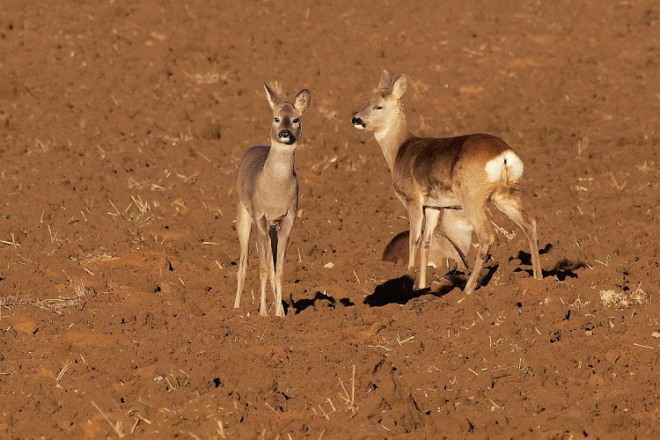
\includegraphics[scale=1.0]{obrazky/ORIGsrnky.jpg}
      \caption{}
    \end{subfigure}
    \begin{subfigure}{0.49\textwidth}
      \centering
      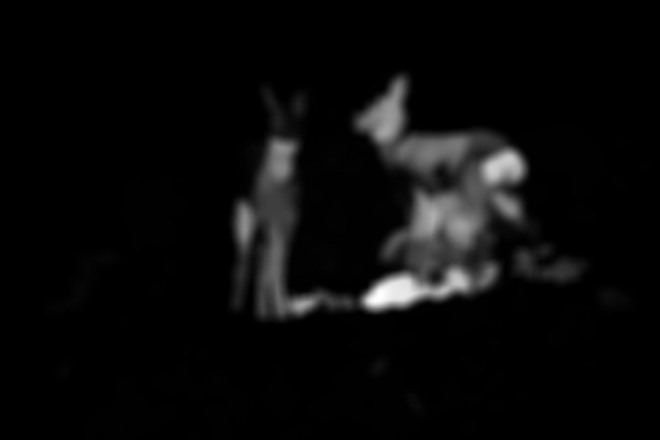
\includegraphics[scale=1.0]{obrazky/MargolinSMsrnky.jpg}
      \caption{}
    \end{subfigure}
    \vspace{4pt}
    
    \begin{subfigure}{0.49\textwidth}
      \centering
      
\includegraphics[scale=1.0]{obrazky/SM8x8.jpg}
      \caption{}
    \end{subfigure}
    \begin{subfigure}{0.49\textwidth}
      \centering
      
\includegraphics[scale=1.0]{obrazky/SM4x4.jpg}
      \caption{}
    \end{subfigure}
    
\caption{(a) Originální fotografie. (b) Vygenerovaná \emph{saliency map} ve stejné velikosti jako originální fotografie. (c) Obrázek \emph{saliency map} o~velikosti 8x8 pixelů(zvětšený). (d) Obrázek \emph{saliency map} o~velikosti 4x4 pixelů(zvětšený).}
\label{obr:spatialpyramid}
\end{figure}

Nyní máme zvoleno kritérium pro reprezentaci kompozice, čímž je výše uvedená víceúrovňová pyramida vytvořená na základě \emph{saliency map}. Dále je nezbytné mít k~dispozici vhodnou sadu fotografií, která by mohla být použita pro trénink tohoto modelu. Tato sada by měla obsahovat velké množství fotografií, které by představovaly fotografie s~dobrou kompozicí a~stejné množství fotografií, které by naopak reprezentovaly špatnou kompozici.

Zatímco fotografie s~dobrou kompozicí lze snadno nalézt na vybraných předních fotografických serverech, tak shromáždit velké množství fotografií s~vyloženě špatnou kompozicí by bylo mnohem náročnější. Proto autoři této metody shromáždili pouze sadu fotografií s~dobrou kompozicí a~z~ní následně pomocí naprosto náhodných ořezů vytvořili sadu obrázků se špatnou kompozicí. Předpokládá se, že tyto náhodné ořezy by měly zajistit dostatečně špatnou kompozici, například oříznutím části významných objektů nebo porušením kompozičních pravidel, které byly na původní fotografii splněny. Právě vytvoření trénovací sady špatných vzorků bez lidského zásahu je jedna z~výhod tohoto modelu.

V~rámci mé práce jsem použil trochu jinou sadu než použili autoři této metody, kteří shromáždili vybrané snímky ze serveru Photo.net\footnote{\url{https://www.photo.net}}. Použil jsem sice jinou sadu asi 2000 fotografií, nicméně jejich kvalita z~pohledu kompozice by mohla být považována za srovnatelnou s~originální sadou. Shromáždil jsem nejlepší snímky za poslední rok ze sítě Reddit\footnote{\url{https://www.reddit.com}} z~několika kategorií, konkrétně CityPorn, EarthPorn, itookapicture, photocritique, WaterPorn a~windowshots\footnote{\url{https://www.reddit.com/r/CityPorn+EarthPorn+itookapicture+photocritique+waterporn+windowshots/top/?sort=top&t=year}}. Tyto obrázky byly hodnoceny početnou komunitou a~jejich motivy jsou rozdílné, což by mělo zajistit potřebnou kvalitu pro vytvoření modelu.

Pro vytvoření ořezů se špatnou kompozicí jsem nepoužil čistě náhodnou variantu generování rámečků ořezu. Zadefinoval jsem jednu podmínku pro omezení velikosti, aby nedocházelo ke generování příliš malých rámečků ořezu a~také jednu podmínku pro vyjmutí větší části významných regionů tak, aby nezůstávaly kompletně v~rámečku ořezu.

Nyní tyto podmínky definujme formálně vztahy \ref{equation:2.8} a~\ref{equation:2.9}. Nejprve si označme celkovou míru významu v~\emph{saliency map} jako $S_{full}$. Poměr míry významu v~rámečku ořezu $S_{crop}$ oproti celkové míře významu $S_{full}$ definujme jako $S_{content}$. Aby byl rámeček považován za špatný ořez, musí být hodnota $S_{content}$ menší než stanovená hodnota $T_{content}$. Podobně označme poměr plochy(počtu pixelů) rámečku ořezu $A_{crop}$ oproti originální fotografii $A_{full}$ jako $S_{area}$. Aby nedocházelo ke generování příliš malých velikostí rámečků, tento poměr $S_{area}$ musí být vyšší než definovaná hodnota $T_{area}$. Hodnoty $T_{content}$ a~$T_{area}$ jsou v~této práci stanoveny empiricky na $0.25$.

\begin{equation} \label{equation:2.8}
S_{content} = \frac{S_{crop}}{S_{full}}, \qquad S_{content} < T_{content} 
\end{equation}
\begin{equation} \label{equation:2.9}
S_{area} = \frac{A_{crop}}{A_{full}}, \qquad S_{area} > T_{area}
\end{equation}

Důvodem pro definici těchto podmínek byla snaha o~zlepšení sady fotografií se špatnou kompozicí. Pokud by byly rámečky ořezu generovány opravdu čistě náhodně, mohlo by někdy dojít k~situaci, že by náhodný rámeček byl velmi podobný referenční fotografii s~dobrou kompozicí. Myšlenka těchto podmínek nepochází z~referenčního článku \cite{Fang2014}, ale z~práce\footnote{\label{fnote}\url{https://github.com/swook/autocrop}} studenta Spolkové vysoké technické školy v~Curychu(ETHZ). Z~této práce jsem čerpal i~některé poznatky související se samotným tréninkem tohoto modelu a~použil je i~ve své implementaci.

\paragraph{}
V~tuto chvíli máme stanovené kritérium pro reprezentaci kompozice, dále máme také připravenou tréninkovou sadu obsahující dobré i~špatné vzorky fotografií a~zbývá již jen provést strojové učení tohoto modelu. Nejprve rozlišíme fotografie z~vytvořené sady do dvou tříd. První třídu(1) budou tvořit originální fotografie se správnou kompozicí a~druhá třída(0) bude tvořena náhodnými ořezy, které reprezentují špatnou kompozici. 

Pro všechny vzorky v~trénovací sadě jsou vytvořeny \emph{saliency maps}, které jsou poté velikostně normalizovány standardem uvedeným výše. Při použití tří-úrovňové pyramidy tedy získáme pro každý vzorek vektor s~21 hodnotami. Tyto vektory se společně s~příslušnými třídami(0--špatná kompozice, 1--dobrá kompozice) použijí pro samotný trénink výsledného modelu.

Tento trénink probíhá pomocí \emph{SVM(Support vector machines)} \cite{LibSVM}, což je metoda strojového učení s~učitelem. Tato metoda se v~oboru počítačového vidění používá velmi často a~slouží především ke klasifikaci konkrétních vzorků. Úlohou \emph{SVM} je nalézt nadrovinu, která rozdělí prostor s~trénovacími daty tak, že data patřící do odlišných tříd leží v~opačných poloprostorech. 

V~samotné implementaci bylo pro trénink \emph{SVM} použito lineární jádro s~parametrem \emph{C}. Především v~implementaci samotného tréninku jsem se hodnotami některých parametrů inspiroval v~již zmíněné práci\textsuperscript{\ref{fnote}}. Nabízela se možnost použití knihovny \emph{LIBSVM} \cite{LibSVM}, nicméně jsem se v~rámci své implementace spokojil s~použitím potřebných funkcí z~\emph{OpenCV}, která je klíčová pro velkou část implementace této práce. V~této knihovně jsou totiž také dostupné třídy pro podporu \emph{SVM}, které z~\emph{LIBSVM} vychází.

Tento model stačí pochopitelně natrénovat pouze jednou a~poté je  možné ho vždy aplikovat pro analýzu konkrétní fotografie. Výsledné skóre \emph{Visual composition modelu} je určeno pomocí \emph{SVR(Support vector regression)}, což je způsob regresní analýzy. Velmi jednoduše řečeno, výsledné skóre kompozice je v~rámci implementovaného modelu přiřazeno do intervalu $\langle -1;1 \rangle$. Hodnota $-1$ zde reprezentuje ideální správnou kompozici a~naopak hodnota $+1$ značí špatnou kompozici. Čím nižší bude hodnota skóre pro rámeček ořezu, tím lepší kompozici rámeček má a~tím lepšího výsledku dosáhne v~tomto modelu. Přímo na těchto hodnotách skóre lze tedy vybrané rámečky ořezu mezi sebou porovnávat a~vybrat tak optimální výsledek z~\emph{Visual composition modelu}.


\subsection{Boundary simplicity model}
Druhým faktorem je zohlednění míry, jakou rámeček pro možný ořez protíná svými okraji výrazné objekty zachycené na fotografii. Při ořezu obrazu je to obvykle nežádoucí, jelikož odstranění částí těchto objektů může způsobit rozptýlení pozornosti diváka a~tedy snížení významu hlavního objektu.

Pro tento faktor je zde vytvořen \emph{model jednoduchosti okrajů (Boundary simplicity model)}. Cílem tohoto modelu je zvolit nejlepší rámeček pro ořez tak, že svými okraji nebude protínat nejlépe žádné hranice objektů na fotografii, respektive hranice s~nejméně významnými hodnotami. \emph{Boundary simplicity model} se jednoduše snaží snížit šanci vedení ořezu skrz objekty, čímž by mohlo dojít k~jejich částečnému oříznutí.

Prakticky je tento model reprezentován vytvořením jednoduché gradientní mapy, která přiřadí hranicím objektů nejvyšší hodnoty a~ostatním stejnorodým částem hodnoty nižší. Příklad takové mapy, která je v~této práci použita, je zobrazena na obrázku \ref{obr:gradient}. Opět zde stačí použít pouze jeden barevný kanál, který spolehlivě umožní označit hranice objektů světlejšími barvami.

\begin{figure}[H]
  \centering
  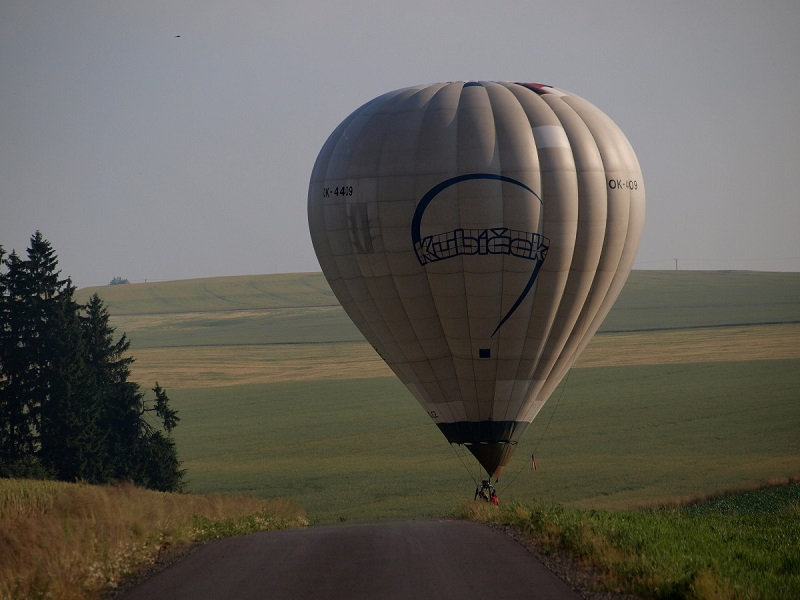
\includegraphics[scale=1.0]{obrazky/ORIGbalon.jpg} \qquad
  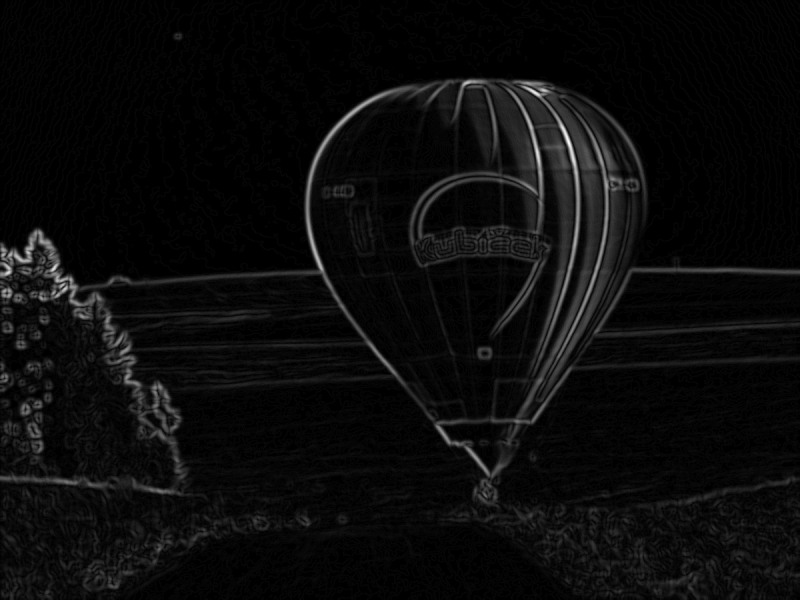
\includegraphics[scale=1.0]{obrazky/gradientbalon.jpg}
  \caption{Vlevo příklad konkrétní fotografie. Vpravo příklad její gradientní mapy, která zvýrazní hrany objektů zachycených na této fotografii.}
  \label{obr:gradient}
\end{figure}

V~této práci uvažujeme klasický rámeček ořezu ve tvaru obdélníku nebo případně čtverce, a~je tedy zřejmé, že bude tvořen 4 stranami, které představují jeho okraje. Výsledek ořezu je tedy vybrán jako rámeček s~nejnižší průměrnou hodnotou z~gradientní mapy v~těchto 4 okrajích. Ve své implementaci jsem použil reprezentaci jednoho okraje šířkou 2 pixely, která se ukázala jako dostačující. Tato šířka představuje silnější reprezentaci než jednoduchá šířka jednoho pixelu. Pochopitelně by mohla být použita ještě větší velikost šířky okraje, nicméně by se tím zbytečně prodlužovala doba výpočtu. Grafická reprezentace okrajů rámečku je znázorněna na obrázku \ref{obr:boundarysimplicitymodel}.

\begin{figure}[H]
  \centering
  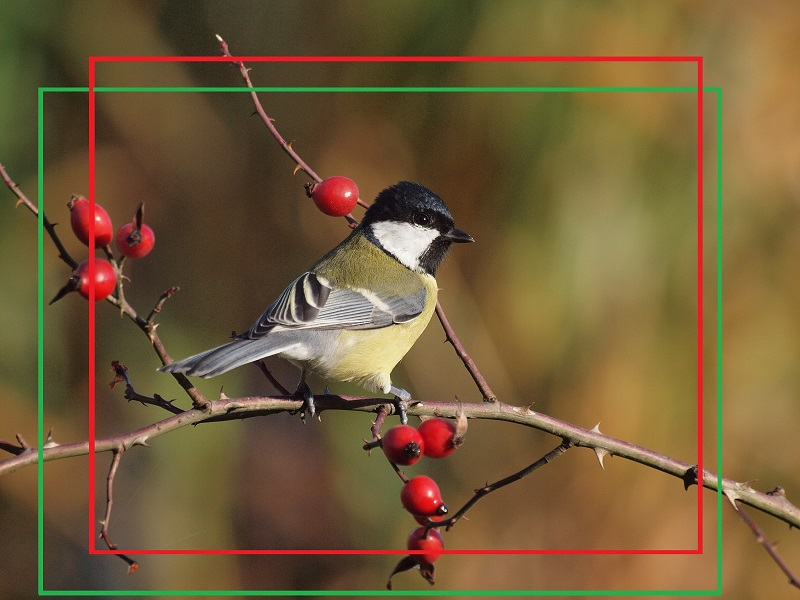
\includegraphics[scale=1.0]{obrazky/sykora-ROIs.jpg} \qquad
  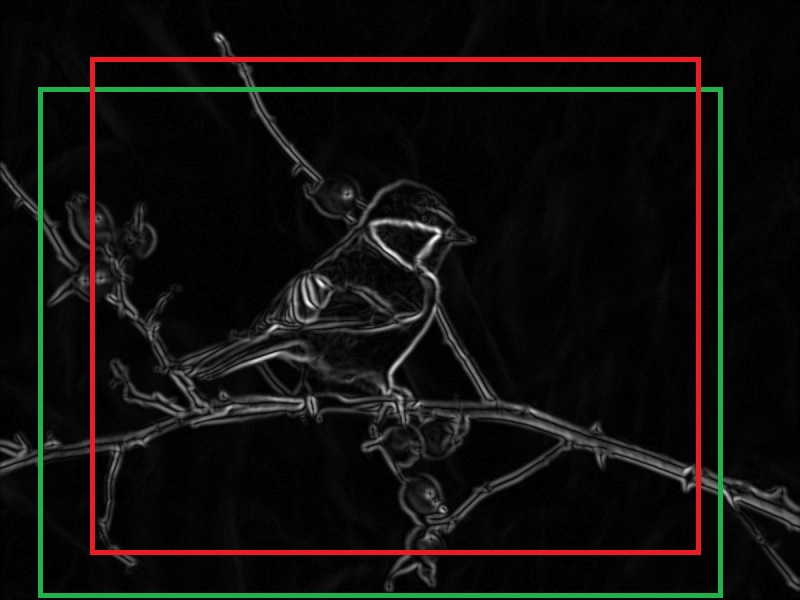
\includegraphics[scale=1.0]{obrazky/sykora-ROIsGrad.jpg}
  \caption{Vlevo je příklad fotografie a~vpravo její gradientní mapa zvýrazňující hranice objektů. Očividně červený rámeček ořezu dosáhne v~rámci tohoto modelu horšího výsledku, protože protíná hned několik hranic objektů. Naopak zelený rámeček jistě bude kvalitnější z~pohledu tohoto modelu, jelikož neprotíná takové množství výraznějších hranic.}
  \label{obr:boundarysimplicitymodel}
\end{figure}

V~mé implementaci je pro vytvoření gradientní mapy použit \emph{Sobelův filtr}. Pro lepší kvalitu gradientní mapy je možné původní fotografii jemně rozmazat a~odstranit tak drobné okraje či nerovnosti, které často nejsou hlavním objektem, například vlny na vodní hladině či stébla trávy na louce. Tohoto rozmazání lze dosáhnout pomocí tzv. \emph{Gaussova filtru}, který umožňuje výrazné odstranění šumu.

\subsection{Content preservation model}
Třetím a~posledním faktorem je zachování hlavního obsahu fotografie. Pro správné zajištění této důležité vlastnosti automatického ořezu je zde vytvořen \emph{model zachování obsahu (Content preservation model)}. Tento model je velmi důležitý, jelikož bez jeho použití bychom mohli dosáhnout ořezů s~dobrou kompozicí, kde by sice hranice rámečku nebyly vedeny skrz objekty, ale tyto ořezy by mohly odstranit hlavní a~významné objekty nebo části.

Jak bude později uvedeno v~popisu samotného algoritmu výběru nejlepšího rámečku ořezu, tento model je použit na úplném začátku procesu. Konkrétně slouží pro odstranění kandidátních rámečků ořezu, které v~sobě nenesou důležité části z~původní fotografie. Tohoto odstranění lze dosáhnout pomocí definice minimální míry významu, kterou v~sobě rámeček ořezu musí nést.

Míra významu je zde opět reprezentována prostřednictvím \emph{saliency map} \cite{Margolin2013}, která významné části detekuje a~zvýrazní. Významnými částmi fotografie jsou myšleny objekty, které přitahují více pozornosti z~hlediska lidského vnímání. Příklad použité \emph{saliency map} je na obrázku \ref{obr:margolinSM}. Významné části jsou opět reprezentovány světlými barvami a~méně důležitý obsah má barvu tmavou. 

Zvolená \emph{saliency map} je pro správnou funkcionalitu tohoto algoritmu automatického ořezu velmi klíčová. Kromě \emph{Content preservation modelu} ji využívá i~\emph{Visual composition model}, jak již bylo zmíněno výše. Celkově vzato je tento model pravděpodobně nejdůležitější ze všech tří uvedených modelů. Rámeček ořezu, který není tímto modelem odstraněn, již může představovat výsledek použitelný z~fotografického hlediska. Výsledky z~předchozích dvou modelů slouží v~podstatě pouze pro vylepšení důležitých detailů a~celkové kvality ořezu.

\begin{figure}[H]
  \centering
  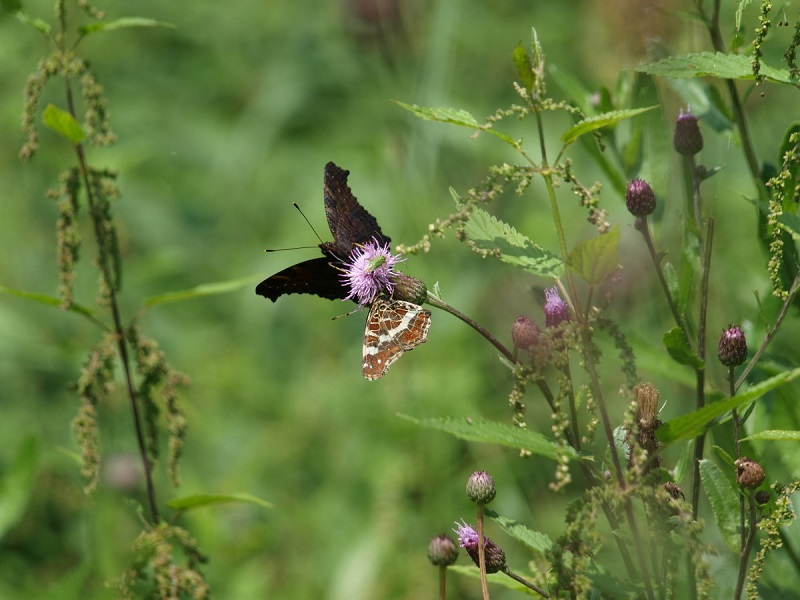
\includegraphics[scale=1.0]{obrazky/ORIGmotyl2.JPG} \qquad
  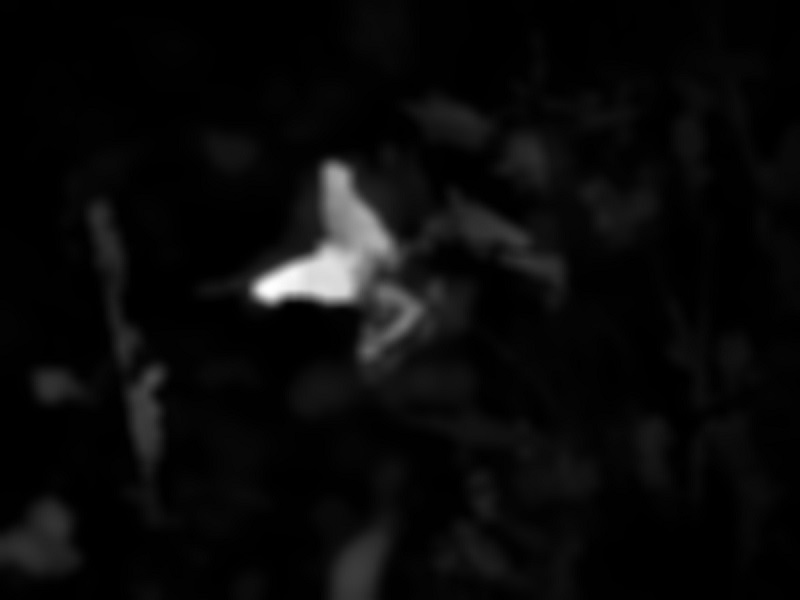
\includegraphics[scale=1.0]{obrazky/MargolinSMmotyl2.jpg}
  \caption{Vlevo je příklad originální fotografie a~vpravo její \emph{saliency map} \cite{Margolin2013}.}
  \label{obr:margolinSM}
\end{figure}


\subsection{Výběr nejlepšího rámečku}
Výběrem nejlepšího rámečku ořezu se zde rozumí proces, který ve výpočtech zohlední všechny výše uvedené modely. Samotný proces výběru nejlepšího rámečku se skládá z~několika po sobě jdoucích kroků.

\begin{enumerate}
\item Prvním krokem je vytvoření základů \emph{Content preservation modelu} a~\emph{Boundary simplicity modelu}. Pro tyto modely je nutné ze vstupní fotografie vytvořit její \emph{saliency map} a~také gradientní mapu. Tyto mapy budou používány během následujících výpočtů.

\item Dále jsou navrženi kandidáti rámečků pro ořez, pro které budou spuštěny výpočty jednotlivých vlastností. Pojmem kandidáti se v~podstatě rozumí parametry či rozměry rámečku. Je nezbytné znát pozici levého horního rohu rámečku, tedy jeho horizontální a~vertikální souřadnice. Dále v~sobě kandidátní rámeček musí nést svoji šířku a~výšku, respektive pozici svého pravého dolního rohu. 

Způsob generování těchto kandidátů může být různý. Rozměry rámečku mohou být například přesně definovány nebo se mohou generovat úplně náhodně. V~takovém případě je ale důležité pamatovat na jistá omezení, aby nemohlo docházet k~vytváření velmi malých rámečků.

\item Nyní je nutné odstranit kandidáty rámečků ořezu, které neobsahují dostatečnou míru významu. Jsou tedy odebráni kandidáti, kteří by případným ořezem odstranili hlavní a~významné části fotografie.

Tohoto lze dosáhnout pomocí \emph{Content preservation modelu}, kde lze empiricky definovat minimální hodnotu míry významu, kterou musí rámeček ořezu mít. Tato hodnota je vypočtena jako poměr míry významu v~daném rámečku oproti míře významu celé fotografie. Jsou odstraněny veškeré rámečky, které zvolené minimální míry nedosahují.

\item Nyní můžeme pracovat už pouze s~kandidáty, které lze považovat za rámečky nesoucí v~sobě dostatečnou míru pozornosti či významu z~původní fotografie. Pro každého ze zbývajících kandidátů je vypočteno výsledné skóre, které závisí na hodnotě získané z~\emph{Boundary simplicity modelu} a~\emph{Visual composition modelu}. Aby bylo možné tyto hodnoty zkombinovat, je potřeba je nějakým způsobem normalizovat. Každému kandidátovi je proto přiřazen údaj, který říká, kolik jiných kandidátů má lepší vlastnost popsanou daným modelem. V~podstatě je vytvořeno pořadí podle skóre z~těchto modelů. 

Označme konkrétního kandidáta, respektive rámeček, jako $C$ a~originální fotografii jako $I$. Hodnotu získanou z~\emph{Visual composition modelu} označme jako $R_{compos} (C, I)$, což je tedy počet všech kandidátů, které dosáhli lepšího výsledku z~hlediska tohoto modelu než rámeček $C$. Obdobně je definována i~hodnota $R_{boundary} (C, I)$, která představuje výsledek podle \emph{Boundary simplicity modelu}. 

Výsledné skóre $S_{final} (C, I)$ je pro každého z~kandidátů vypočítáno jako lineární kombinace těchto hodnot, kde lze navíc přiřadit hodnotám získaných z~modelů i~různé váhové koeficienty. S~těmito váhami je možné experimentovat a~sledovat jejich vliv na výsledky ořezu pro různé typy fotografií, čemuž se budeme podrobněji věnovat v~sekci \ref{sekce:expmetody}. Formálně je tento výpočet popsán rovnicí \ref{equation:2.10}. Optimálním rámečkem je zvolen kandidát, který dosáhl celkově nejlepšího výsledku $S_{final} (C, I)$.

\begin{equation} \label{equation:2.10}
S_{final} (C, I) = w1 R_{compos} (C, I) + w2 R_{boundary} (C, I)
\end{equation}
\end{enumerate}

Na obrázku \ref{obr:modelsCrop} je ukázka rozdílu mezi ořezem vybraným pouze na základě výsledného skóre z~\emph{Content preservation modelu} a~ořezem vypočítaným na základě spojení mezi \emph{Content preservation} a~\emph{Boundary simplicity modelem}. Konkrétně pro tento případ byli nejprve vybráni kandidáti rámečku ořezu, kteří dosáhli dostačujícího výsledku v~\emph{Content preservation modelu}, tedy měli dostatečnou míru významu podle \emph{saliency map}. Poté byl nejlepší rámeček vybrán pouze na základě skóre v~\emph{Boundary simplicity modelu}, tedy tak, aby protínal co nejméně výrazných hranic objektů.

\begin{figure}[H]
    \centering
    \begin{subfigure}{0.32\textwidth}
      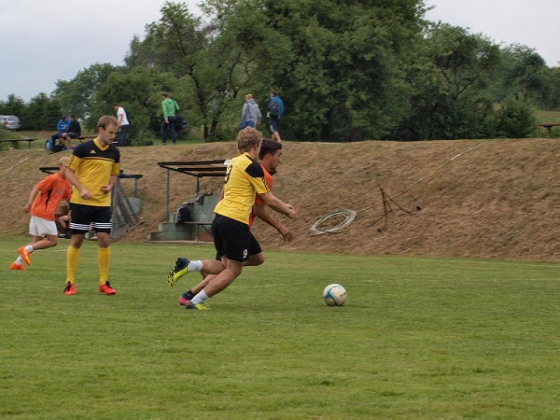
\includegraphics[scale=1.0]{obrazky/ORIGfotbal1.jpg}
      \caption{}
    \end{subfigure}
    \begin{subfigure}{.32\textwidth}
      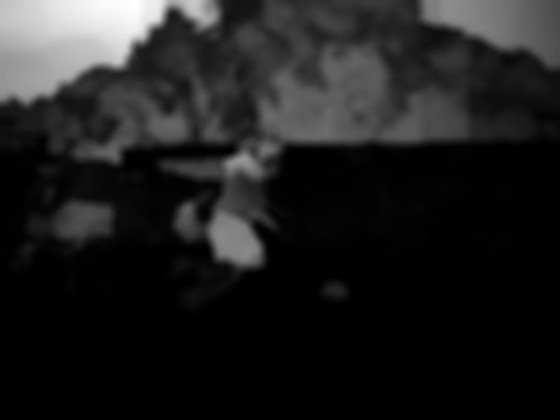
\includegraphics[scale=1.0]{obrazky/MargolinSMfotbal1.jpg}
      \caption{}
    \end{subfigure}
    \begin{subfigure}{.32\textwidth}
      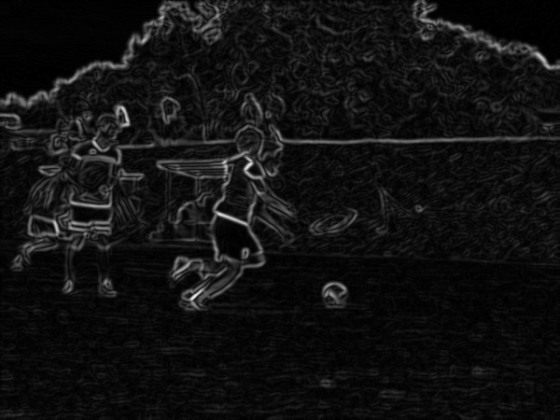
\includegraphics[scale=1.0]{obrazky/gradientfotbal1.jpg}
      \caption{}
    \end{subfigure}
    \vspace{2pt}
    
    \begin{subfigure}{0.3\textwidth}
      \centering
      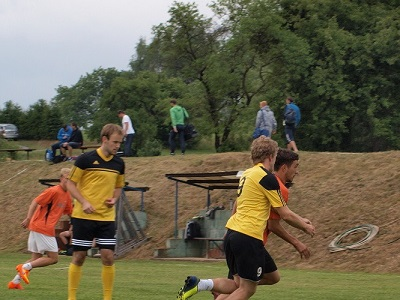
\includegraphics[scale=1.0]{obrazky/crop2fotbal1.jpg}
      \caption{}
    \end{subfigure}
    \begin{subfigure}{.3\textwidth}
      \centering
      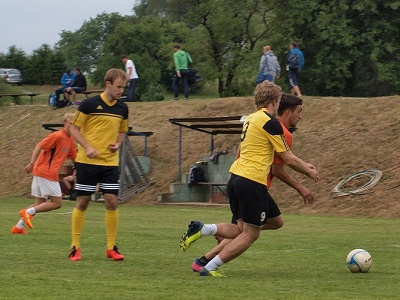
\includegraphics[scale=1.0]{obrazky/crop2fotbal1-simplicity.jpg}
      \caption{}
    \end{subfigure}
    
\caption{(a) Originální fotografie.
(b) \emph{Saliency map} \cite{Margolin2013} této fotografie(\emph{Content preservation model}) 
(c) Gradientní mapa se~zvýrazněním hran objektů na fotografii(\emph{Boundary simplicity model})
(d) Ořez se zmenšením velikosti fotografie na 2/3 původní velikosti podle nejlepšího výsledku pouze z~analýzy saliency mapy (\emph{Content preservation model)}. 
(e) Ořez se zmenšením velikosti fotografie na 2/3 původní velikosti podle nejlepšího výsledku spojení \emph{Content preservation modelu} a~\emph{Boundary simplicity modelu}}
\label{obr:modelsCrop}
\end{figure}

Výběr nejlepšího rámečku na obrázku \ref{obr:modelsCrop} ještě žádným způsobem neovlivnilo skóre získané z~\emph{Visual composition modelu}. Pro kompletní výsledek automatického ořezu musíme ale toto skóre zahrnout přesně podle rovnice \ref{equation:2.10}, kde je možné nastavit váhové koeficienty pro význam obou modelů. Na obrázku \ref{obr:allModelsCrop} jsou již zahrnuty veškeré skóre, a~váhy jsou nastaveny na 5 pro \emph{Visual composition model} a~na 1 pro \emph{Boundary simplicity model}. Toto nastavení by mělo podle článku \cite{Fang2014} dávat nejlepší výsledky. Kandidáti rámečků jsou zde generováni na různých pozicích a~v~různých velikostech.

\begin{figure}[H]
	\centering
    \begin{subfigure}{0.32\textwidth}
   	  \centering
      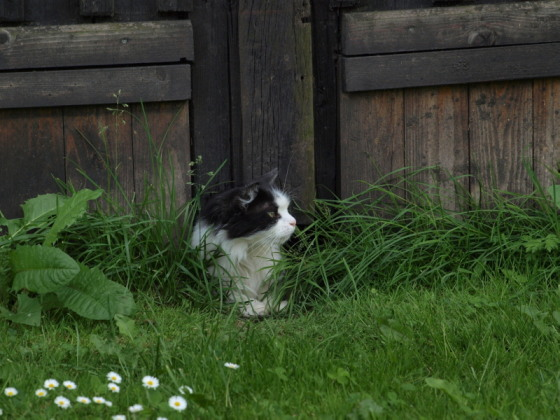
\includegraphics[scale=1.0]{obrazky/ORIGlecian.jpg}
    \end{subfigure}
    \begin{subfigure}{.32\textwidth}
      \centering
      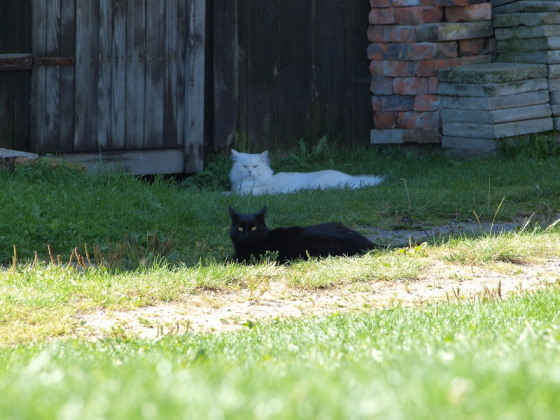
\includegraphics[scale=1.0]{obrazky/ORIGkocky.jpg}
    \end{subfigure}
    \begin{subfigure}{.32\textwidth}
      \centering
      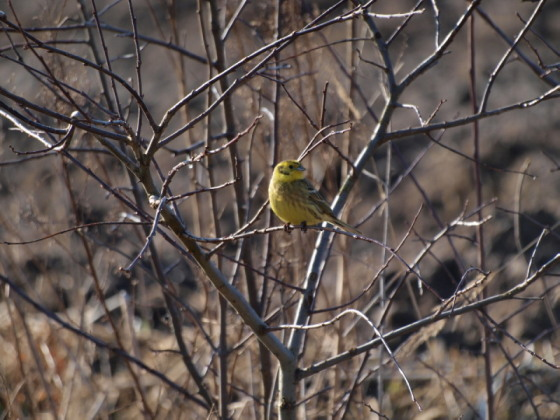
\includegraphics[scale=1.0]{obrazky/ORIGstrnad.JPG}
    \end{subfigure}
    \vspace{2pt}
    
    \begin{subfigure}{0.32\textwidth}
      \centering
      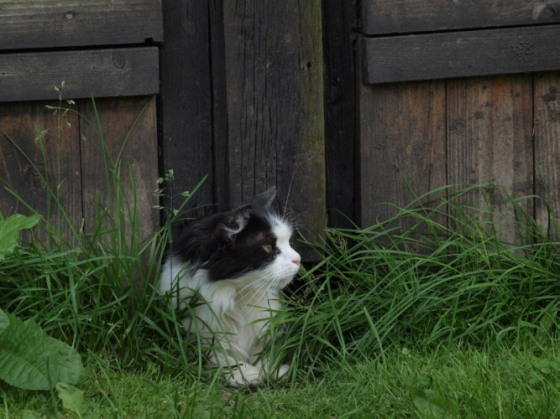
\includegraphics[scale=1.0]{obrazky/cropFanglecian.jpg}
    \end{subfigure}
    \begin{subfigure}{.32\textwidth}
      \centering
      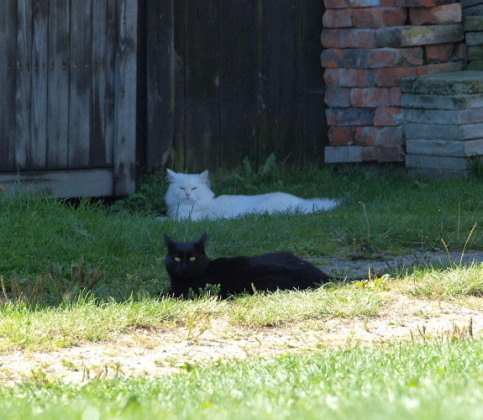
\includegraphics[scale=1.0]{obrazky/cropFangkocky.jpg}
    \end{subfigure}
    \begin{subfigure}{.32\textwidth}
      \centering
      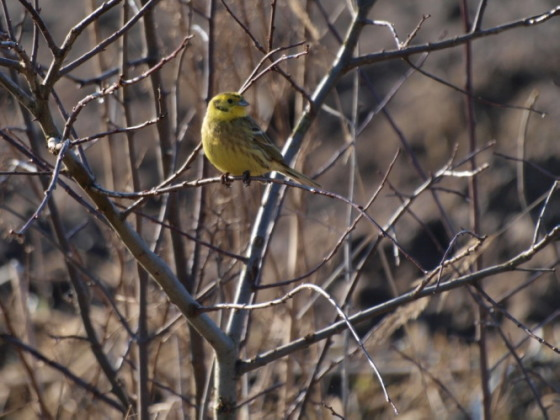
\includegraphics[scale=1.0]{obrazky/cropFangstrnad.jpg}
    \end{subfigure}
    \vspace{1pt}
\caption{Nahoře jsou originální fotografie a~dole jejich ořezy, které byly vytvořeny přesně podle popisu této metody automatického ořezu \cite{Fang2014}.}
\label{obr:allModelsCrop}
\end{figure}

Výhodou této metody je jistě její robustnost, jelikož zohledňuje hned tři důležité faktory, které ovlivňují kvalitu výsledného ořezu. Tato vybraná metoda automatického ořezu obrazu \cite{Fang2014} by měla dosahovat nejlepších výsledků v~rámci zvolených metod v~této bakalářské práci.

Nevýhodou této metody by v~některých situacích mohla být použitá \emph{saliency map} \cite{Margolin2013}. Mohlo by se například stát, že by nefungovala přesně a~přiřadila by vyšší hodnoty míry významu pro jiné části než pro hlavní objekty. Tím pádem by v~podstatě znehodnotila výsledky v~rámci \emph{Content preservation modelu} a~\emph{Visual composition modelu}. Nicméně použití \emph{saliency map} toto riziko v~sobě nese i~v~jiných algoritmech automatického ořezu fotografií. Tento problém bude podrobněji diskutován v~sekci \ref{sekce:expmetody}.
\newpage


%------------------ SECTION ---------------------%
\section{Automatic Thumbnail Cropping and its Effectiveness}\label{sekce:metoda3}
Nejstarší zvolená metoda automatického ořezu \cite{Suh2003} vznikla v~době, kdy začalo být aktuální nějakým způsobem vytvořit menší náhled(\emph{thumbnail}) určitě větší fotografie. Používání náhledů je pochopitelně aktuální i~v~současné době, kdy se s~nimi denně setkáváme na internetu nebo během používání různých přístrojů, které mají omezenou velikost obrazovky. 

Obrázek náhledu by měl už na první pohled divákovi sdělit, co je hlavním předmětem obrázku. Někdy pochopitelně stačí originální obrázek zmenšit na maximální možnou velikost náhledu. Existuje ovšem spousta situací, kdy v~takovém případě není v~náhledu jasně patrné, co se na obrázku nachází a~objekty nelze jednoduše rozeznat. Proto je často používán pro vytváření náhledu kromě zmenšení i~ořez. Právě ořez obrázku pro vytvoření náhledu je hlavní motivací této metody. Cílem je tedy v~podstatě prezentovat divákovi obrázek náhledu tak, aby byla už na první pohled zřejmá hlavní podstata originálního obrázku.

Tato metoda automatického ořezu přichází s~obecným řešením, které je založeno na míře pozornosti a~významu jednotlivých objektů na fotografii. Konkrétně je zde pro reprezentaci této míry použita \emph{saliency map} \cite{Itti1998}. Tato \emph{saliency map} v~podstatě představuje model lidské vizuální pozornosti při vnímání obrázků. Jednoduše lze říci, že \emph{saliency map} zastupuje důležitost a~význam všech pozic na originální fotografii. Rámeček ořezu v~sobě tedy ponese požadovanou část míry významu z~originální fotografie a~díky tomu může přiblížit hlavní objekty.

\subsection{Saliency map}
Stejně jako v~předešlých dvou zvolených algoritmech automatického ořezu, je i~pro tuto metodu potřebné mít k~dispozici \emph{saliency map} reprezentující význam částí fotografie. V~tomto případě se jedná konkrétně o~dnes již historickou \emph{saliency map} z~roku 1998 \cite{Itti1998}. Jak jsem měl možnost zjistit, tak tato metoda generování \emph{saliency map} funguje velmi dobře i~v~případech, kdy hlavní objekty nejsou příliš výrazné oproti jejich okolí na originální fotografii, což je pro algoritmus automatického ořezu klíčové. Dobrých výsledků je dosaženo především díky kombinaci důležitých faktorů, které umožňují odhalit různorodé prvky zachycené na fotografii. Tyto faktory budou v~této podsekci stručně popsány.

Ještě před popisem vlastností této \emph{saliency map} bych chtěl uvést na pravou míru způsob její implementace v~této práci. V~tomto případě jsem se inspiroval existujícími implementacemi\footnote{\url{https://github.com/akisato-/saliencyMap}}\footnote{\url{https://github.com/akisato-/pySaliencyMap}}, na jejichž základě jsem vytvořil vlastní implementaci. Z~těchto implementací jsem odstranil všechny přebytečné funkce a~konstanty, které nebyly podstatné pro generování \emph{saliency map} použitou pro algoritmus automatického ořezu. Dále jsem provedl úpravy, díky kterým byly tyto implementace prakticky převedeny do zvyklostí C++ a~aktuální verze 3.4 knihovny \emph{OpenCV}. Nakonec jsem v~implementaci změnil i~několik částí, které se lišily od původního popisu \cite{Itti1998}.

\begin{figure}[H]
	\centering
    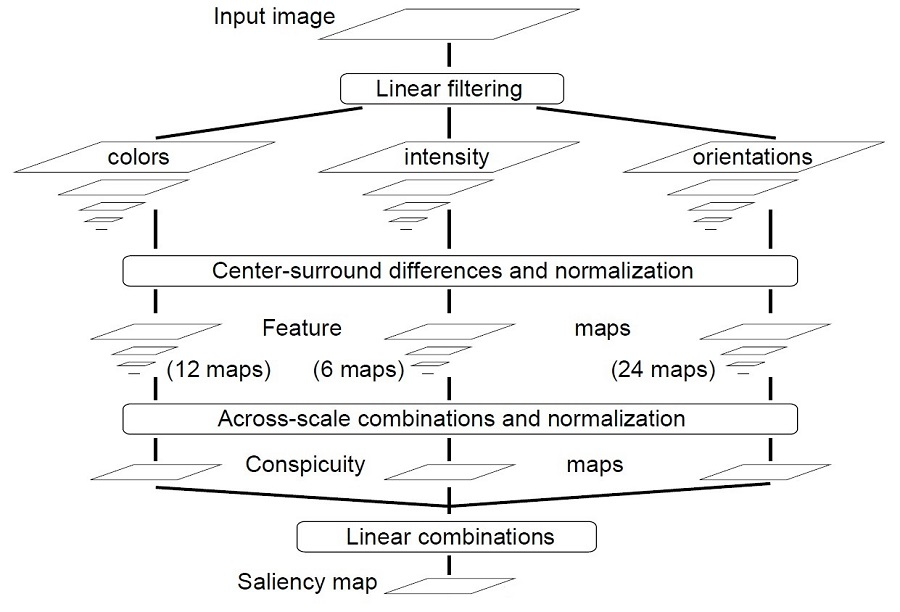
\includegraphics[scale=0.75]{obrazky/itti_schema.jpg}
    \caption{Schéma modelu generování uvedené \emph{saliency map} \cite{Itti1998}}
    \label{obr:itti_schema}
\end{figure}

Tato metoda nejdříve z~originálního obrázku extrahuje jednotlivé kanály barev $R,G,B$ a~také kanál intenzity $I$, který je získán jednoduše průměrováním barevných kanálů. Pro faktor intenzity je vytvořena 9-úrovňová pyramida, kde první stupeň tvoří matice intenzity ve stejné velikosti jako je originální obrázek a~kde každý další stupeň této pyramidy je zmenšen na polovinu velikosti předchozího stupně. Při využití této pyramidové technologie je třeba pamatovat na to, aby se vždy při zmenšování aktuálního stupně provedlo jeho rozmazání a~také vzorkování. Kromě pyramidy pro intenzitu jsou vytvořeny i~další 9-úrovňové pyramidy pro jednotlivé barevné kanály $R,G,B$ a~také pro kanál žluté barvy $Y$, který je vypočítán podle konkrétní rovnice \cite{Itti1998}.

Pro tyto pyramidy jsou provedeny \emph{center-surround} operace, které představují klíčový princip výzkumu provedeného v~referenční práci \cite{Itti1998}. Pomocí nich lze totiž odhalit části fotografie, které se z~daného hlediska liší od jejich okolí. Na jejich základě je vytvořeno celkem 6 \emph{feature maps} pro reprezentaci intenzity a~12 \emph{feature maps} pro získání informace o~rozdílu barevných složek. 

Posledním faktorem je informace o~lokální orientaci částí fotografie, která je získána z~vytvořené pyramidy intenzity. Pro její výpočet je nutné využít tzv. \emph{Gaborových filtrů} pro různé směry. V~jejich přesné definici a~použití jsem se inspiroval v~již uvedené existující implementaci. Pro tento faktor orientace je vytvořeno 24 \emph{feature maps}. 

Dohromady je tedy vygenerováno 42 \emph{feature maps}, jak je uvedeno na schématu \ref{obr:itti_schema}. Pro tyto \emph{feature maps} je dále použit normalizační operátor a~následně jsou normalizované mapy zkombinovány. Jednotlivým faktorům je možné pro kombinaci přiřadit různou důležitost pomocí váhových koeficientů, nicméně podle referenční metody mají mít tyto faktory nastavenou stejnou váhu. Na základě kombinace všech uvedených faktorů je vytvořena finální \emph{saliency map}, která může být použita pro aplikaci algoritmu automatického ořezu. 

Veškeré části generování této \emph{saliency map} jsem zde popsal velmi stručně. Bylo by jistě možné uvést kromě tohoto krátkého slovního popisu i~všechny potřebné rovnice, nicméně ty je možné nalézt v~referenčním článku \cite{Itti1998}. V~tomto článku je vše podstatné velmi podrobně vysvětleno a~nepovažoval jsem proto za nezbytné tyto informace přesně opisovat. Naopak v~sekci \ref{section:metoda1} jsem provedl detailnější popis generování \emph{saliency map}, jelikož v~referenčním článku \cite{Stentiford2007} jsou některé části vysvětleny jen okrajově a~nemusí být tedy zřejmé, jak jsem je ve své práci použil.

Postup vytváření použité \emph{saliency map} je znázorněn na obrázku \ref{obr:ittiSM}, kde jsou uvedeny výsledky jednotlivých map pro zmíněné faktory a~také finální výstup \emph{saliency map} pro zadanou fotografii.

\begin{figure}[H]
	\centering
    \begin{subfigure}{\textwidth}
   	  \centering
      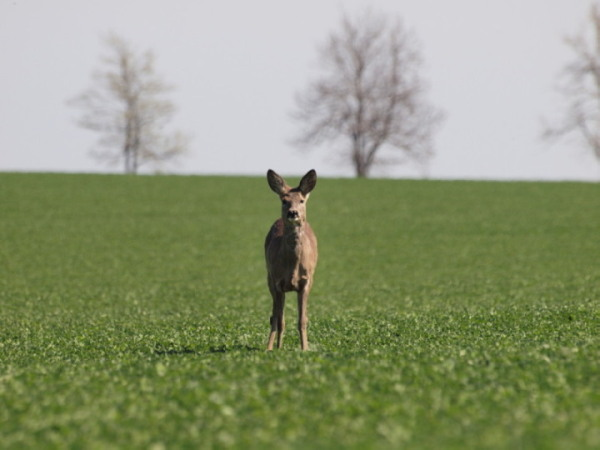
\includegraphics[scale=1.0]{obrazky/ORIG23.jpg}
      \caption{}
    \end{subfigure}
    \vspace{2pt}
    
    \begin{subfigure}{.32\textwidth}
      \centering
      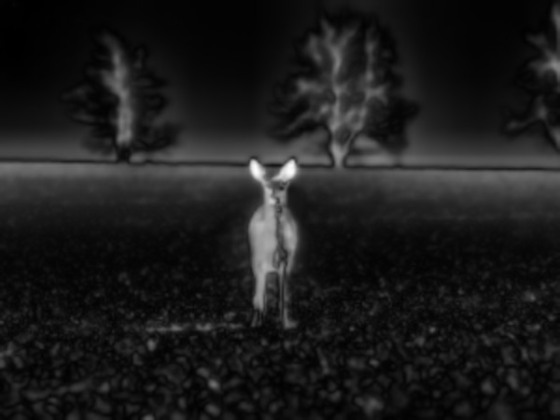
\includegraphics[scale=1.0]{obrazky/ittiIntensity23.jpg}
      \caption{}
    \end{subfigure}
    \begin{subfigure}{.32\textwidth}
      \centering
      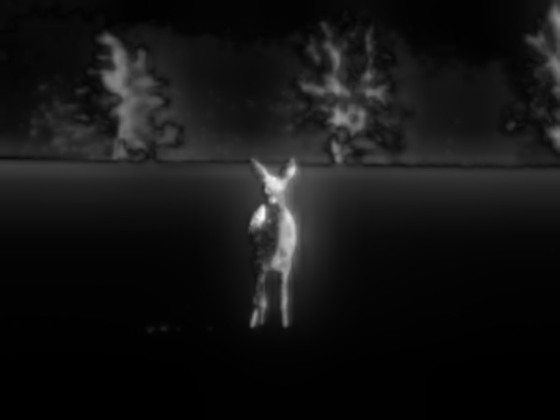
\includegraphics[scale=1.0]{obrazky/ittiColour23.jpg}
      \caption{}
    \end{subfigure}
    \vspace{2pt}
    \begin{subfigure}{0.32\textwidth}
      \centering
      \includegraphics[scale=1.0]{obrazky/ittiOrientation23.jpg}
      \caption{}
    \end{subfigure}
    \vspace{2pt}
    
    \begin{subfigure}{\textwidth}
      \centering
      \includegraphics[scale=1.0]{obrazky/ittiSM23.jpg}
      \caption{}
    \end{subfigure}
\caption{(a) Originální fotografie. (b) Normalizovaná mapa pro reprezentaci faktoru intenzity. (c) Normalizovaná mapa pro reprezentaci rozdílů barevných složek. (d) Normalizovaná mapa pro reprezentaci orientace lokálních částí. (e) Výstupní \emph{saliency map} získaná kombinací výše uvedených map.}
\label{obr:ittiSM}
\end{figure}


\subsection{Výběr rámečku hrubou silou s~pevným prahem}
Pro začátek popisu tohoto algoritmu ořezu si definujeme úlohu výběru obecně tak, jak je popsán v~této metodě. Označíme originální obrázek jako  $I$. Cílem algoritmu ořezu je nalézt oblast zájmu, která má tvar obdélníku a~obsahuje hlavní objekty originálního obrázku $I$. Tuto oblast, respektive rámeček, označíme jako $R_C$. Po ořezu oblasti zájmu je možné ji ještě zmenšit pro obrázek náhledu $I_C$, který může mít přesné rozměry výšky a~šířky.

Jak již bylo zmíněno výše, tak tato metoda obecně používá pro reprezentaci míry významu hodnoty získané ze \emph{saliency map} $S_I$. Rámeček ořezu $R_C$ by měl splnit dvě hlavní podmínky, tedy mít co nejmenší velikost a~zároveň obsahovat co největší část významných objektů z~originálního obrázku $I$. Tyto podmínky se ale v~podstatě vzájemně vylučují, proto se tato metoda se snaží nalézt rámeček, který by je dokázal částečně vyrovnat a~představoval by mezi nimi optimální kompromis.

\paragraph{}
Součet míry významu jednotlivých pixelů v~\emph{saliency map} $S_I$, které jsou součástí oblasti zájmu $R_C$, by měl být pochopitelně co nejvyšší. Na základě tohoto předpokladu tento algoritmus hledá co nejmenší rámeček, který má požadovanou hodnotu míru významu. Zmíněná hodnota je vypočtena jako poměr součtu míry významu uvnitř $R_C$ a~součtu celkové míry významu obrázku $I$, respektive $S_I$. 

Formálně označme pole obsahující kandidáty na hledaný rámeček $R_C$ 
jako $\Re(\lambda)$. $\lambda$ je prahová hodnota minimální poměru, kterou musí výše zmíněný poměr součtu míry významu možného rámečku $r$ a~celkového součtu míry v~obrázku přesáhnout, aby mohl být daný rámeček $r$ zařazen mezi kandidáty. 

\begin{equation} \label{equation:2.11}
\Re(\lambda) = \left\{ r: \frac{\sum\limits_{(x,y) \in r}{S_I(x,y)}}{\sum\limits_{(x,y)}{S_I(x,y)}} >\lambda \right\}
\end{equation}

\begin{equation} \label{equation:2.12}
R_C = \argmin_{r \in \Re(\lambda)}(area(r))
\end{equation}

Rovnice \ref{equation:2.11} formálně definuje pole kandidátů rámečku ořezu $\Re(\lambda)$, tedy všech rámečků, které mají dostatečnou míru významu. Rovnice \ref{equation:2.12} pak určuje, že optimální rámeček $R_C$ bude vybrán jako nejmenší rámeček z~pole kandidátů $\Re(\lambda)$.

Výpočet hledání rámečku zde probíhá tzv. brutální silou. V~praxi to znamená, že jsou na každé pozici postupně vytvářeny rámečky různých velikostí a~pro každý z~nich je vypočtena míra významu $S_I$ na základě \emph{saliency map}. V~tomto způsobu výběru rámečku je pochopitelně lepší začít s~generováním rámečku o~co nejmenší velikosti. Následně se budou postupně provádět výpočty pro hledání rámečku, který by splňoval minimální prahovou hodnotu míry významu $\lambda$. Pokud by tato míra významu definovaná prahovou hodnotou nebyla pro danou velikost nalezena, byla by velikost rámečku určitým způsobem zvětšena a~takto by se pokračovalo, dokud by nebyl požadovaný rámeček ořezu nalezen. Díky tomuto způsobu je tedy možné dosáhnout kompromisu mezi požadovanou mírou významu a~velikostí rámečku.

Návrhy implementace, které by mohly nějakým způsobem zefektivnit algoritmy výpočtu hrubou silou, budou uvedeny později v~sekci \ref{sekce:navrh_metody}. Příklad ořezu této metody je graficky znázorněn na obrázku \ref{obr:suhCrop}, kde byla pevně stanovena prahová hodnota a~výpočet probíhal hrubou silou.

\begin{figure}[H]
    \centering
    \begin{subfigure}{0.32\textwidth}
      \centering
      \includegraphics[scale=1.0]{obrazky/ORIG31.jpg}
    \end{subfigure}
    \begin{subfigure}{.32\textwidth}
      \centering
      \includegraphics[scale=1.0]{obrazky/ittiSM31.jpg}
    \end{subfigure}
    \begin{subfigure}{.32\textwidth}
      \centering
      \includegraphics[scale=1.0]{obrazky/cropSuh31.jpg}
    \end{subfigure}
    \vspace{2pt}
    
    \begin{subfigure}{0.32\textwidth}
      \centering
      \includegraphics[scale=1.0]{obrazky/ORIG35.jpg}
      \caption{}
    \end{subfigure}
    \begin{subfigure}{.32\textwidth}
      \centering
      \includegraphics[scale=1.0]{obrazky/ittiSM35.jpg}
      \caption{}
    \end{subfigure}
    \begin{subfigure}{.32\textwidth}
      \centering
      \includegraphics[scale=1.0]{obrazky/cropSuh35.jpg}
      \caption{}
    \end{subfigure}
    \vspace{1pt}
    
\caption{(a) Originální fotografie. (b) \emph{Saliency map} \cite{Itti1998} pro jednotlivé fotografie. (c) Automatický ořez \cite{Suh2003}, který nalezl rámeček s~minimální velikostí při poměru stran 3:2(prahová hodnota $\lambda$ byla nastavena na hodnotu 0.7).}
\label{obr:suhCrop}
\end{figure}

\subsection{Výběr rámečku hladovým algoritmem s~pevným prahem}
Algoritmus hrubou silou pracuje sice spolehlivě, nicméně je časově neefektivní. Proto tato metoda sama definuje použití tzv. \emph{hladového(greedy) algoritmu}, který využívá hledání maximálních hodnot míry významu v~\emph{saliency map}. I~když v~některých případech není výsledek výběru rámečku tak přesný jako v~případě použití metodu hrubé síly, je tento algoritmus časově efektivnější a~zároveň spolehlivě nalezne hlavní objekty z~původního obrázku. Tento způsob výběru je tedy výraznou optimalizací rychlosti hledání požadovaného rámečku ořezu.

Hladový algoritmus provádí výpočet oblasti zájmu, respektive rámečku $R_C$, na základě nalezení pixelu $P$ s~maximální hodnotou míry významu. Jeho princip je znázorněn v~algoritmu \ref{algoritmus:greedy}. Nejdříve je nutné inicializovat pozici rámečku $R_C$, která je nastavena přesně do středu \emph{saliency map} $S$. Tato inicializace vychází z~předpokladu, že ve většině případů bude hlavní objekt umístěn přibližně ve středu původní fotografie, případně v~jeho okolí. Samozřejmě se mohou objekty vyskytovat blíže k~některému okraji originální fotografie, ale i~pro tyto situace by měl způsob výběru hladovým algoritmem nalézt řešení.

Vždy se bude hledat pixel $P$, který leží mimo rámeček $R_C$ a~který má maximální hodnotu míry pozornosti v~\emph{saliency map} $S$. Kolem tohoto pixelu bude vytvořen menší obdélník $R^{\prime}$, jelikož je velmi pravděpodobné, že pixel $P$ bude součástí některého hlavního objektu a~menší oblast kolem tohoto pixelu bude zřejmě také obsahovat část objektu. Poté je třeba aktualizovat rámeček $R_C$ tak, že je původní oblast $R_C$ sjednocena s~obdélníkem $R^{\prime}$. Dále je proveden výpočet míry významu v~$R_C$, a~pokud je tato míra dostatečná, je algoritmus ukončen. Během výpočtu se tedy bude postupně zvyšovat velikost rámečku $R_C$, dokud nebude dosaženo požadované hodnoty míry významu.

\paragraph{}
\begin{algorithm}[H]
\SetAlgorithmName{Algoritmus}{}
 RRámeček HLADOVY\_OREZ $(S, \lambda)$
 
 $tresholdSuma \leftarrow \lambda$ * Celková hodnota míry významu v~$S$\;
 $R_C \leftarrow$ Střed saliency map $S$\;
 $aktualniMiraVyznamu \leftarrow$ Hodnota míry významu v~$R_C$\;
 \While{$aktualniMiraVyznamu < tresholdSuma$} {
  $P \leftarrow$ Pixel s~nejvyšší hodnotou míry významu mimo $R_C$\;
  $R^{\prime} \leftarrow$ Malý obdélník se středem $P$\;
  $R_C \leftarrow$ UNION$(R_C, R^{\prime})$\;
  Aktualizace $aktualniMiraVyznamu$ na novou hodnotu v~$R_C$\;
 }
 \Return $R_C$\;
 
 \caption{Hladový algoritmus\cite{Suh2003} pro nalezení rámečku ořezu s~pevným prahem míry významu. $S$ je \emph{saliency map} a~$\lambda$ je stanovený práh.}
 \label{algoritmus:greedy}
\end{algorithm}

\paragraph{}
Autoři této metody také zkoumali optimální prahovou hodnotu míry významu, která je potřebná pro výběr rámečku ořezu. Optimální hodnota je pro každou fotografii různá a~její efektivní stanovení by mohlo výrazně zlepšit rychlost výpočtu a~rovněž i~celkový výsledek ořezu. Způsob nalezení této efektivní prahové hodnoty je přesně uveden v~referenčním článku \cite{Suh2003}. Spočívá v~tom, že tato efektivní hodnota je nalezena jako bod, od kterého dochází k~co nejmenšímu nárůstu míry významu a~zároveň velkému zvyšování velikosti rámečku. Tento způsob se velmi hodí použít ve chvíli, kdy nemáme představu o~tom, jakou prahovou hodnotu bychom měli stanovit.

V~referenčním článku tohoto algoritmu automatického ořezu \cite{Suh2003} autoři také vyzkoušeli provedení výběru rámečku na základě detekce obličejů. Poté experimentovali s~výsledky ořezy dosaženými pro sady různých typů fotografií. Mohli tak demonstrovat, že metoda postavena na detekci obličejů funguje pro automatický ořez fotografií osob či portrétů lépe než obecná metoda, kterou jsem popsal v~mé práci. Tuto metodu založenou na detekci obličejů jsem v~této práci nevyzkoušel jednak z~časových důvodů a~jednak z~jejího úzkého zaměření pro konkrétní typy fotografií. Nicméně by určitě mohlo být zajímavé ji implementovat během budoucí práce.

Celkově tato obecná metoda automatického ořezu umožňuje provádět výběr rámečku tak, že v~něm zachová jeho podstatné části. Díky použité \emph{saliency map} lze tyto části velmi dobře nalézt. Výsledek tohoto algoritmu automatického ořezu velmi závisí na požadováné míře významu, pro kterou musí být definovaná prahová hodnota. Na jejím základě je pak zvolen co nejmenší rámeček ořezu, který představuje lepší prezentaci originální fotografie například v~obrázku náhledu. Nevýhodou této metody je fakt, že žádným způsobem nezohledňuje kompozici výsledného ořezu. Výsledky ořezu proto nemusí působit úplně harmonicky, jelikož objekty v~rámečku ořezu mohou být poskládány neočekávaným způsobem.

%================== CHAPTER =====================%
\chapter{Návrh a~implementace}
V~této kapitole bude popsán postup návrhu implementace zvolených metod pro automatický ořez fotografií. V~předchozí kapitole bylo již zmíněno velké množství obecných způsobů, které jsem ve své implementaci použil. Zde budou upřesněny především principy vytvořených funkcí, které jsem prakticky implementoval. Během návrhu je dobré prostudovat již existující nástroje, jelikož by mohly pomoci k~inspiraci pro různé varianty použití vybraných algoritmů automatického ořezu.

%------------------ SECTION ---------------------%
\section{Existující řešení}
\label{sekce:3.1}
Většina editorů fotografií umožňuje široké spektrům úprav. Ořez mezi tyto úpravy pochopitelně patří, jelikož se skutečně jedná o~jednu ze základních a~nejdůležitějších technik úpravy fotografií. Velká část editorů ovšem neposkytuje funkci automatického ořezu obrazu. Touto funkcí editoru je myšleno automatické nalezení optimálního rámečku ořezu, například na základě přesně zadané velikosti šířky a~výšky, nebo zadaného poměru velikosti mezi šířkou a~výškou rámečku. 

Podařilo se mi najít a~vyzkoušet několik volně dostupných řešení, z~nichž bych zde stručně některé popsal. Tyto nástroje používají vlastní algoritmy pro nalezení nejlepšího ořezu a~v~budoucnu by bylo možné jejich výstupy porovnat s~metodami automatického ořezu, které jsem implementoval.

\subsection{Cropp.me}
První aplikací, kterou jsem vyzkoušel, byla webová aplikace \emph{Cropp.me}\footnote{\url{http://cropp.me}}. Jedná se o~jednoduchou aplikaci, která se zaměřuje přímo na automatický ořez fotografií. Umožňuje nahrát fotografii na server, dále definovat šířku a~výšku výsledného rámečku nebo si vybrat z~nabídky doporučených rozměrů. Následně je proveden automatický ořez a~výstupní fotografie je možné si stáhnout, respektive uložit. Velkou výhodou této aplikace je rychlé dosažení poměrně dobrých výsledků.

Během experimentování s~touto aplikací jsem byl přesvědčen, že výsledné ořezy v~téměř všech případech obsahovaly hlavní objekty z~původní fotografie. Konkrétní algoritmus automatického ořezu, který tato aplikace používá, se mi nepodařilo zjistit. Tato aplikace je poměrně omezená z~hlediska opakovaného používání. Zdarma je možné nahrát pouze omezený počet fotografií denně i~měsíčně. Pro větší množství je nutné se zaregistrovat a~zaplatit si tarif. I~tak oceňuji jednoduchost a~moderní uživatelské rozhraní této webové aplikace.

\subsection{Croppola.com}
Jedná se webovou aplikaci\footnote{\url{https://croppola.com}}, která primárně umožňuje automatický ořez fotografií. Na základě nahrané vstupní fotografie je proveden velmi rychlý výpočet, který uživateli vykreslí do originálního obrázku rámeček pro případný ořez. Je možné si vybrat z~nabídky nejčastěji používaných rozměrů rámečku podle poměru mezi jeho šířkou a~výškou. Kromě nejčastěji používaných poměrů jsou zde uvedeny také specifické poměry, které používá například \emph{Facebook} či \emph{Twitter} pro velikosti profilových či úvodních fotografií.

Po provedení návrhu automatického ořezu aplikace navíc poskytuje možnost si rámeček ještě manuálně přizpůsobit, respektive posunout nebo změnit jeho velikost. Tato možnost je řešena velmi elegantně pomocí webových technologií a~řada uživatelů ji jistě ocení. Algoritmus automatického ořezu, který \emph{croppola} používá, totiž v~některých případech nefunguje úplně přesvědčivě, což jsem zjistil při pokusech ořezů náhodně vybraných fotografií. 

Výsledné ořezy je možné si stáhnout a~uložit. Tato aplikace mě zaujala díky intuitivnímu uživatelskému rozhraní a~oceňuji i~velmi rychlý způsob výpočtu používaného algoritmu automatického ořezu.

\subsection{Autosplitter}
Tato desktopová aplikace\footnote{\url{https://autosplitter.com}} umožňuje načíst obrázek a~provést jeho rychlou analýzu. Na základě této analýzy automaticky detekuje jeden či více rámečků, které obsahují významnou část na originální fotografii. Výhodou je možnost analyzovat více fotografií současně a~také možnost manuální úpravy navrženého rámečku ořezu. Automaticky vygenerované rámečky jsou často velmi malé velikosti, takže obsahují prakticky jen detekovaný objekt.

Kromě možnosti automatické detekce výrazných částí a~návrhu rámečků ořezu tento software také poskytuje další funkce jako je změna barevného vyvážení fotografie. \emph{Autosplitter} nepřináší lepší výsledky oproti webovým aplikacím uvedeným výše, naopak navržené rámečky ořezu jsou z~fotografického hlediska často mnohem horší. Tuto aplikaci jsem vyzkoušel pouze v~její zkušební verzi, jelikož plnou verzi je nutné si zakoupit.

\subsection{Twitter}
Fakt, že se s~automatickým ořezem obrázků setkáváme v~podstatě každý den, si možná ani neuvědomujeme. Většina sociálních sítí, kde je možné sdílet obrázky, totiž často využívá automatický ořez pro zobrazení nejdůležitějších částí nahraných obrázků. Uživatelé mohou na sociální sítě nahrávat obrázky nejrůznějších rozměrů a~poměrů stran. Aby obsah těchto sítí vypadal při prohlížení hlavních stránek dobře, jsou zde definované standardy poměrů stran, v~jakých se obrázky náhledů zobrazují. Při kliknutí na tento náhled lze často zjistit, že originální obrázek má vlastně úplně jiný poměr stran, než měl zobrazený náhled. I~tak je žádoucí, aby na zobrazeném náhledu byly zobrazeny všechny podstatné části.

Jako příklad si uveďme jednou z~nejznámějších sociálních sítí, která umožňuje sdílení fotografií. Touto populární sítí je \emph{Twitter}\footnote{\url{https://twitter.com}}, kam denně miliony lidí přidávají své fotografie. Právě \emph{Twitter} používá vlastní algoritmy pro automatický ořez fotografií\footnote{\url{https://blog.twitter.com/engineering/en_us/topics/infrastructure/2018/Smart-Auto-Cropping-of-Images.html}}. V~letošním roce je jejich nový algoritmus nasazován a~určitě bude ještě nějakým způsobem dále vyvíjen. Je zřejmé, že především pro tyto oblasti je problematika automatického ořezu velmi aktuální. Na těchto algoritmech může být stále více vlastností optimalizováno či vylepšeno a~právě tyto problémy jsou dobrou motivací pro další výzkum v~oblasti automatického ořezu fotografií.

%------------------ SECTION ---------------------%
\section{Návrh implementace metod pro automatický ořez}
\label{sekce:navrh_metody}
V~této sekci nebudou popsány konkrétní algoritmy metod automatického ořezu, které již byly popsány v~kapitole \ref{chapter:2}. Bude zde uveden návrh implementace funkcí, které byly v~rámci každého vybraného algoritmu automatického ořezu vytvořeny a~také si uvedeme důvody jejich vytvoření.

\subsection{Typy funkcí automatického ořezu}
Základní funkcí by mělo být nalezení optimálního rámečku ořezu na originální fotografii podle přesného zadání rozměrů jeho šířky a~výšky. Předpokladem pro tuto funkci je situace, kdy uživatel potřebuje z~nějakého důvodu oříznout fotografii na přesný rozměr. Příkladem by mohl být požadavek nahrávání fotografie na nějaký server, kde by byl nastaven maximální limit rozměrů fotografie a~uživatel chtěl zachovat co nejvyšší velikost rozměrů. Díky této funkci lze navíc vybrané algoritmy automatického ořezu mezi sebou dobře porovnávat, jelikož každá metoda s~nejvyšší pravděpodobností vybere rámeček ořezu na jiné pozici, což závisí na konkrétních vlastnostech.

Další funkcí by měla být možnost hledat optimální rámeček na základě vzájemného poměru šířky a~výšky výstupní fotografie. Uživatel by mohl chtít u~výstupní fotografie zachovat tento poměr stejný jako u~originálu. V~takovém případě by se jednalo pouze o~zmenšení originální fotografie a~bylo by možné zadávat, kolikrát má být výstup ořezu menší oproti originálu, respektive kolikrát má být originální fotografie větší oproti výstupní. V~tomto případě se tedy opět jedná o~funkci s~přesnou definicí rozměrů, ovšem zde by navíc zůstal zachován původní poměr rozměrů rámečku.

Jiná funkce související s~poměrem rozměrů fotografie bere v~potaz možnost, že uživatel nepožaduje zachování poměru mezi šířkou a~výškou, ale naopak potřebuje specifikovat konkrétní poměr. Například by tedy mohl požadovat, aby šířka a~výška výstupní fotografie byla v~poměru 4:3. V~takové situaci bude hledán optimální rámeček, který by tento poměr dodržel. Nicméně v~této situaci je velmi vhodné definovat hranici velikosti, kterou by rozměry výstupního ořezu neměly přesáhnout. Touto hranicí je myšlena minimální a~případně i~maximální šířka či výška obrázku.

Důvodem pro definování hranic při tomto způsobu hledání je především fakt, že vybrané metody automatického ořezu mohou konvergovat k~velmi nepřesnému řešení. K~tomuto by mohlo dojít například v~situaci, kdy by byl oříznut velmi malý rámeček, protože by splňoval výsledky definovaných výpočtů algoritmu automatického ořezu nejlépe. Jak již bylo zmíněno dříve, při použití první vybrané metody\cite{Stentiford2007} by mohla být vybrána jen velmi malá část na základě nejvyšších hodnot míry významu použité \emph{saliency map}. Například by tak mohlo být vybráno jen lidské oko, i~když by hlavní podstatou fotografie byl velký portrét obličeje.

Také jsem se pro každou metodu automatického ořezu implementoval funkce, které by všechny předchozí funkce ve své podstatě zaobalily. Tyto funkce by měly na základě zadané originální fotografie navrhnout jednoho nebo několik vhodných kandidátů, které by mohly být považovány za kvalitní ořezy použitelné z~fotografického hlediska. V~těchto funkcích se hledají rámečky různých rozměrů šířky i~výšky, a~zároveň i~jejich vzájemných libovolných poměrů. Výhodou těchto funkcí je možnost jejich použití bez specifikace konkrétních parametrů, kterými jsou právě šířka a~výška.

Pro tento typ funkcí je vždy třeba zvolit pravidla, podle kterých se budou generovat pozice a~velikosti rámečku, pro které budou dále vypočteny jejich výsledky algoritmů automatického ořezu. Hodnoty těchto pozic mohou být generovány například úplně náhodně, čímž lze často dosáhnout překvapivě dobrých výsledků ořezu. Aby byla šance, že takové metody uspějí, je nezbytné definovat již zmíněné hraniční hodnoty pro minimální velikost rámečků ořezu. 

\subsection{Způsoby výpočtu výběru nejlepšího rámečku}
Ve všech třech implementovaných algoritmech automatického ořezu \cite{Fang2014,Stentiford2007,Suh2003} je možné aplikovat různé možnosti generování rámečků, pro které bude vypočítáno výsledné skóre. V~referenčních článcích je sice definován obecný způsob výpočtu skóre pro konkrétní rámeček, který je často zapsán pomocí vztahů a~rovnic, ale přesný způsob navrhování pozic a~rozměrů rámečku se zde již neřeší. Právě tyto způsoby návrhu rámečků jsem v~rámci programové části této práce sám navrhl a~implementoval je.

Než se budeme věnovat samotným variantám generování, popišme si nyní jednoduché parametry rámečku, které jsou nezbytné pro jeho definici. Tyto parametry jsou v~podstatě pouze 4. První dva z~nich jsou horizontální a~vertikální souřadnice levého horního rohu rámečku. Důvod, proč volíme levý horní roh a~nikoliv některý jiný z~rohů, je prostý. Spočívá v~tom, že souřadný systém načtených obrázků je indexován také z~levého horního rohu. Jednoduše pixel, který bude umístěn v~levém horním rohu na načtené originální fotografii, bude umístěn na souřadnici $[0;0]$. Kromě pozice levého horního rohu potřebujeme znát i~parametry pro šířku a~výšku rámečku, respektive pozici pravého dolního rohu rámečku. Tyto parametry v~sobě musí obsahovat každý rámeček a~možné varianty pro jejich získání budou nyní popsány.

\paragraph{}
Nejprve si popišme možnosti návrhu pozic levého horního rohu rámečku. Pokud máme zadanou originální fotografii o~určité velikosti, je možné generovat pozici na každém pixelu originální fotografie a~poté spustit výpočet skóre pro daný rámeček. Toto je v~podstatě nejzákladnější varianta návrhu pozice, nicméně je časově velmi neefektivní. V~případě, kdy je zadána fotografie velké velikosti, by tento výpočet trval velmi dlouho. Proto je lepší negenerovat tyto pozice na každém pixelu, ale pouze na určitých místech.

Pokud si zvolíme hodnotu, která bude definovat vzdálenost mezi navrženými pozicemi v~horizontálním i~vertikálním směru, můžeme vytvořit v~podstatě pravidelnou mřížku. Pokud by tedy byla tato vzdálenost horizontálně i~vertikálně určena hodnotou 10 pixelů, výpočet by se pak 100násobně zrychlil. I~když by se mohlo zdát, že by v~takovém případě byl ořez nepřesný, opak je pravdou. U~větších fotografií lidské oko v~podstatě nepozná výrazný rozdíl oproti procházení po jednom pixelu, u~menších fotografií by i~v~případě vzdálenosti 10 pixelů byl ořez poměrně přesný. Většina implementovaných funkcí v~sobě proto má možnost parametricky určit hodnoty vzdálenosti pro konstrukce této mřížky.

Druhou možností, jak pozice levého horního rohu rámečku vytvářet, je použití náhodného generátoru. V~tom případě je samozřejmě nezbytné definovat i~omezení hodnot pro toto náhodné generování. Definice minimální velikosti rámečku je prakticky vhodná ve všech případech, jak už bylo několikrát zmíněno. V~případě náhodného generování pozic pro horizontální i~vertikální souřadnice lze dosáhnout poměrně dobrých výsledků, přičemž se provede často mnohem méně výpočtů než například při generování pozic v~sestavené mřížce zmíněné výše. Tyto poznatky jsem získal při vlastním testování parametrů mé implementace.

Zbylé dva parametry rámečku, kterými jsou jeho šířka a~výška, mohou být přesně zadány a~není nutné je nějakým způsobem vytvářet. Byly implementovány funkce, kde mohou být šířka a~výška rámečku přesně definovány a~také funkce, kde jsou vypočteny podle zadaného parametru pro zmenšení a~zachování původního poměru rozměrů fotografie. Dále byly implementovány funkce, kde je požadován konkrétní poměr rozměrů rámečku, a~v~těchto případech stačí náhodně nebo podle určitého pravidla určit například hodnotu šířky a~na základě zadaného poměru dopočítat výšku. Také jsem implementoval funkce, kde jsou rozměry rámečku ořezu generovány náhodně. I~u~těchto funkcí lze při dobře definovaných omezeních získat velmi dobré výsledky.

\paragraph{}
U~druhé uvedené metody automatického ořezu \cite{Fang2014} je přesný způsob výpočtu závislý na skóre získaném z~jednotlivých modelů, a~tak rychlost výpočtu závisí především na zvolené metodě generování pozic a~rozměrů, které byly zmíněny výše. U~dalších dvou vybraných algoritmů automatického ořezu \cite{Stentiford2007,Suh2003} je celkový výsledek vypočítán pouze na základě hodnot míry významu z~použitých \emph{saliency maps}. Právě v~těchto případech se nabízí použít různé optimalizace způsobu výpočtu.

V~rámci poslední metody jsem proto vyzkoušel implementovat hladový algoritmus, který byl detailně popsán v~sekci \ref{sekce:metoda3}. Díky tomuto způsobu je možné nalézt poměrně dobrý výsledek, který obsahuje hlavní objekty. Jeho výhodou je především časová efektivita, která je mnohem lepší než u~metod výpočtu hrubou silou. Metody výpočtu nejlepšího rámečku hrubou silou pracují jednoduše tak, že je nutné pro každý vygenerovaný rámeček vypočítat výsledek na základě hodnot ze \emph{saliency map}, přičemž je čtena hodnota míry významu pro všechny pixelu v~rámečku.

Nicméně metody výpočtu hrubou silou pracují dobře i~spolehlivě. Pokud je navíc zvolena vhodná metoda pro generování pozic levého horního rohu rámečku, je i~výsledný čas výpočtu velmi rychlý a~díky tomu lze nalézt dobrý výsledek ořezu použitelný z~fotografického hlediska.

Veškeré funkce a~varianty automatického ořezu, které jsem vytvořil, jsem se snažil v~programové části přehledně komentovat, aby byla zřejmá jejich přesná činnost. I~když jsou si v~některých částech vzájemně podobné, zastřešují všechny situace popsané výše. Jelikož byly tyto funkce vytvořeny pro všechny vybrané algoritmy automatického ořezu, bylo možné díky nim experimentovat a~porovnávat dosažené výsledky pro zadané parametry. Díky tomu šlo lépe posoudit vlastnosti těchto algoritmů automatického ořezu.
\newpage

%------------------ SECTION ---------------------%
\section{Použité technologie}
V~této sekci budou uvedeny technologie, které byly použity pro vypracování programové části této bakalářské práce. Znalost jednotlivých technologií je důležitá pro pochopení způsobu vytváření konkrétních funkcí a~metod. U~každé technologie budou zmíněny hlavní~výhody, které byly rozhodující pro zvolení dané technologie. V~této práci jsem se snažil vybrat známé a~aktuální technologie tak, aby mohl být případný budoucí vývoj jednodušší.

Výsledný program byl vyvíjen a~testován na Ubuntu 16.04 a~také ve vývojovém prostředí Microsoft Visual Studio 2017 na platformě Windows 10. Pro sestavení spustitelné aplikace byl použit překladový nástroj CMake\footnote{\url{https://cmake.org}}. Pro úspěšné přeložení a~spuštění aplikace je nutné mít všechny technologie uvedené v~této sekci správně nainstalovány.

\subsection{C++}
Jedná se o~programovací jazyk, který vznikl jako rozšíření jazyka C. Jazyk C++ není jazykem čistě objektově orientovaným, jelikož podporuje několik dalších programovacích stylů, jako je generické programování a~procedurální programování. V~současné době patří jazyk C++ mezi nejrozšířenější a~nejpoužívanější programovací jazyky.

Velkou výhodou tohoto jazyka jsou i~jeho rozsáhlé standardy\footnote{\url{https://isocpp.org}}, které se neustále vyvíjí. Programovou část této práce jsem vytvořil tak, aby byla kompatibilní se standardem C++11. V~současné době je nejnovějším standardem C++17.

\subsection{OpenCV}
Knihovna \emph{OpenCV(Open Source Computer Vision Library)}\footnote{\url{https://opencv.org}} je zveřejněna pod BSD licencí a~je tedy volně dostupná pro akademické i~komerční použití. Jedná se o~multiplatformní knihovnu dostupnou pro systémy Windows, Linux, MacOS a~Android. Poskytuje rozhraní pro Python, Javu a~C++. Právě rozhraní pro jazyk C++ bylo v~této práci použito.

\emph{OpenCV} byla navržena pro výpočetní efektivitu se zaměřením na real--time aplikace. Knihovna je napsána v~jazycích C a~C++ v~optimalizované podobě. V~této práci je použita její aktuální verze \emph{OpenCV} 3.4. Z~této knihovny jsem použil především její algoritmy počítačového vidění aplikovatelné pro 2D prostor, a~také jsem ji využil při implementaci metody strojového učení \emph{SVM(Support Vector Machines)}. Tato knihovna byla klíčová pro vytvoření velké části uvedených metod.

\subsection{VLFeat}
\emph{VLFeat} je open--source knihovna\footnote{\url{http://www.vlfeat.org}}, která implementuje některé známé algoritmy z~oblasti počítačového vidění. Tato knihovna je napsána v~jazyce C, především z~důvodu výkonosti a~kompatibility. Jedná se o~multiplatformní knihovnu, která je podporována systémy Windows, Mac OS a~Linux. 

V~této bakalářské práci byla použita aktuální verze \emph{VLFeat} 0.9.21. Konkrétně zde byla tato knihovna aplikována pro implementaci superpixelů \emph{SLIC}, které byly součástí implementace \emph{saliency map} \cite{Margolin2013} použité v~druhé uvedené metodě automatického ořezu \cite{Fang2014}.

\subsection{Boost}
\emph{Boost}\footnote{\url{http://www.boost.org}} je knihovna pro programovací jazyk C++. Je tvořena množstvím různých typů knihoven, mezi které patří například knihovny pro zpracování obrazu, regulárních výrazů či práci se souborovým systémem. Boost je multiplatformní knihovna, která je podporována systémy typu UNIX, Windows i~Mac OS. Část knihoven, které \emph{Boost} nabízí, byla dokonce standardizována ve standardu C++11 a~některé další části byly standardizovány nedávno v~C++17. Boost je licencován pod vlastní open-source licencí. V~této práci byla použita její verze 1.67.0. 

Z~této knihovny jsem použil funkce umožňující načítání souborů z~konkrétních adresářů. Toto načítání bylo velmi užitečné při extrakci informace o~kompozici fotografií, které byly potřebné pro trénink \emph{Visual composition modelu} ze druhé metody automatického ořezu \cite{Fang2014}. V~tomto případě bylo potřeba načíst fotografie s~dobrou vlastností kompozice ze sady asi 2100 obrázků, které byly uloženy ve stejném adresáři, což knihovna \emph{Boost} výrazně zjednodušila.

%================== CHAPTER =====================%
\chapter{Testování a~experimenty}
Tato kapitola popisuje návrh a~realizaci testování výstupů zvolených metod automatického ořezu fotografií. Implementované metody byly porovnány formou uživatelského testování, na jehož základě zde bude provedena diskuze.

Dále budou uvedeny vlastní experimenty, které jsem během implementace jednotlivých metod vyzkoušel. Na základě experimentů budou názorně demonstrovány některé důležité vlastnosti. Také budou předvedeny příklady fotografií, pro které algoritmy automatického ořezu nezafungovaly správně a~bude rozebrán důvod jejich selhání.

%------------------ SECTION ---------------------%
\section{Testování výstupů metod pro automatický ořez}
V~této sekci bude popsáno testování výsledků automatického ořezu fotografií především z~fotografického úhlu pohledu. Cílem bylo vytvořit uživatelské testování, v~rámci kterého byly vybrané metody mezi sebou porovnány. Jednalo se o~kvantitativní porovnání, a~proto bylo vhodné do tohoto testu přidat dostatečné množství ořezů a~také zapojit co nejvíce lidí.

\subsection{Návrh a~realizace testování}
Nejdříve bylo nutné zvolit systém či formu uživatelského testování. V~tomto případě se jednalo o~porovnávání automatických ořezů jednotlivých algoritmů. Jelikož se snažíme dosáhnout kvantitativního porovnání metod, tak by bylo vhodné, aby porovnávání mohlo probíhat jednoduše a~zároveň rychle.

Úkolem porovnání je v~podstatě seřadit výstupy v~takovém pořadí, jak se líbí uživateli. Pokud by uživatel musel seřadit například 4 obrázky v~pořadí od nejlepšího k~nejhoršímu, tak by pro něj rozhodování mohlo být velmi zdlouhavé a~také obtížné, protože se obrázky často mohou lišit jen malými detaily. Pokud by se ale člověk mohl vždy rozhodnout pouze mezi dvěma obrázky, bylo by to pro něj mnohem jednodušší i~rychlejší.

Existuje metoda, která umožňuje toto porovnání provádět postupným výběrem mezi dvojicemi obrázků. Tato psychofyzikální rozhodovací metoda se nazývá \emph{Two-alternative forced choice(2AFC)} \cite{David1988}. Uživateli se postupně zobrazují dva obrázky v~náhodném pořadí a~jeho úkolem je vybrat právě jeden z~nich. Během tohoto rozhodování hraje svou roli i~čas, za který je uživatel schopen zvolit lepší obrázek. Rozhodovacímu času jsem ale v~rámci tohoto testování nepřiřadil klíčovou roli.

\paragraph{}
Zvolili jsme tedy formu testování a~dále bylo nezbytné vybrat vhodná data, které pro testování použijeme. Smyslem ořezu je vylepšit původní fotografii, čehož lze dosáhnout například přiblížením hlavního objektu či odstraněním rušivých prvků. Na základě tohoto předpokladu bylo zvoleno 20 fotografií, jejichž kvalita by mohla být pomocí ořezu zlepšena. Vybrané fotografie měly různé motivy, aby testování bylo více objektivní. Jednalo se například o~fotografie zvířat, přírody, lidí, sportu nebo budov.

Pro každou z~vybraných fotografií byly provedeny automatické ořezy pomocí všech tří implementovaných algoritmů \cite{Fang2014,Stentiford2007,Suh2003}. Kromě toho jsem také požádal fotografa s~mnohaletými zkušenostmi, aby provedl ořezy všech 20 fotografií manuálně. Je nezbytné upřesnit, že se nejednalo o~profesionálního fotografa, ale o~člověka, pro kterého je fotografování hlavním koníčkem. Pro každou originální fotografii vznikly celkem 4 ořezy, které byly předmětem porovnávání.

Vzniklo tak 20 sad obrázků, které obsahovaly 3 automatické ořezy a~jeden manuální ořez. Podle rozhodovací metody 2AFC je celkový počet porovnání v~jedné sadě roven počtu $n*(n-1)/2$, kde $n$ je počet porovnávaných ořezů. V~našem případě se v~rámci jedné sady provede 6 porovnání. Pro 20 sad je to tedy celkem už 120 párových porovnání. Toto jednoduché porovnání je pro představu znázorněno na obrázku \ref{obr:TestUkazka2}.

Kromě tohoto základního porovnání, kdy jsou zobrazeny pouze samotné dva ořezy, jsem také vytvořil druhou část testu, kde byla zobrazena i~referenční fotografie. Tato referenční fotografie byla zobrazena vždy uprostřed mezi ořezy(viz obrázek \ref{obr:TestUkazka3}). Bylo proto vytvořeno dalších 20 sad, které obsahovaly stejné ořezy a~referenční fotografii. V~celkovém součtu tedy uživatelé museli pro úspěšné dokončení testu provést 240 porovnání. Motivací pro vytvoření testovacích sad s~referenční fotografií byla především snaha o~zjištění, jak velké rozdíly budou tyto sady ve výsledku mít oproti sadám, kde se zobrazí pouze samotné dva ořezy.

\begin{figure}[H]
	\centering
	\includegraphics[scale=1.0]{obrazky/TEST2.jpg}
	\caption{Ukázka párového testu dvou ořezů, kde uživatel zvolí lepší obrázek.}
\label{obr:TestUkazka2}
\end{figure}

\begin{figure}[H]
	\centering
	\includegraphics[scale=1.0]{obrazky/TEST3.jpg}
	\caption{Ukázka párového testu dvou ořezů, mezi nimiž je zobrazena původní fotografie.}
\label{obr:TestUkazka3}
\end{figure}

Pro samotnou realizaci párového testování jsem použil webový nástroj \cite{Sevcik2015}, který mi dodal vedoucí práce. Pomocí tohoto nástroje jsem vytvořil sady s~ořezy tak, jak bylo zmíněno výše. Také jsem mohl přidat jednoduché a~srozumitelné pokyny, které byly uživatelům zobrazeny před zahájením testu. Dále jsem vytvořil krátký dotazník, který uživatel vyplnil na konci testu. 

Tento webový nástroj jsem nahrál na server, a~mohl tak uživatelům zasílat test v~podobě URL odkazu. Uživatel již nemusel nic instalovat a~mohl přímo vybírat lepší ořez pomocí kliknutí myši nebo stisknutím šipek na klávesnici. Tato skutečnost byla velkou výhodou, díky které se testování mohlo zúčastnit větší množství lidí.


\subsection{Výsledky testování}
Test úspěšně dokončilo 57 lidí. Několik uživatelů test kompletně nedokončilo, a~tak jejich výsledky byly smazány z~důvodu vyšší přesnosti výsledků. Tento počet tvořilo 34 mužů a~23 žen, mezi které patřili zástupci všech generací. Nicméně velkou část testovaných představovali studenti, a~proto byl celkový věkový průměr zúčastněných 23,92 let. 

Průměrná délka testování byla přibližně 22 minut, a~průměrná rozhodovací doba uživatele pro jedno porovnání byla 5,2 vteřin. Zde je třeba zmínit, že rozhodovací doba se ve většině případů pohybovala přibližně kolem 3 vteřin. Nicméně v~některých případech zde byly zaznamenány časy v~řádů desítek až stovek vteřin, což bylo pravděpodobně způsobeno problémy s~připojením nebo přestávky uživatele. Z~tohoto důvodu nelze vyvodit přesné závěry pro rozhodovací časy.

Celkové výsledky součtů výběru jednotlivých metod ve všech 40 sadách, tedy 20 sadách se zobrazenou referenční fotografií a~20 sadách bez zobrazení referenční fotografie, jsou zobrazeny na obrázku \ref{obr:TestTotal}. Manuální ořez dosáhl celkem 20krát nejvyššího hodnocení, tedy zvítězil přesně v~polovině sad. Druhá vybraná metoda \cite{Fang2014} zvítězila celkem v~8 sadách. Třetí implementovaná metoda \cite{Suh2003} zvítězila v~7 sadách a~Stentifordova metoda \cite{Stentiford2007} dosáhla nejlepších výsledků pouze 5krát. Počty nejlepších výsledků pro jednotlivé metody jsou zobrazeny v~následující tabulce.

\begin{table}[H]
	\centering
    \begin{tabular}{| l | l | l | l | l |}
    \hline
    Počet nejlepších výsledků& Manuální & Fang et al. \cite{Fang2014} & Stentiford F. \cite{Stentiford2007} & Suh et al. \cite{Suh2003} \\ \hline
    sady bez reference & 9 & 4 & 3 & 4 \\ \hline
    sady s~referencí & 11 & 4 & 2 & 3 \\ \hline
    celkově & 20 & 8 & 5 & 7 \\ 
    \hline
    \end{tabular}
    \caption{Tabulka počtu nejlepších výsledků v~rámci různých sad.}
    \label{tab:test}
\end{table}

\begin{figure}[H]
	\centering
	\includegraphics[scale=0.6]{obrazky/TESTtotal.png}
	\caption{Celkové výsledky získané ze všech sad.}
\label{obr:TestTotal}
\end{figure}

\begin{figure}[H]
	\centering
	\includegraphics[scale=0.6]{obrazky/TESTwithoutRef.png}
    \caption{Výsledky získané za sad obrázků, kde byly uživateli zobrazeny vždy pouze samotné dva ořezy.}
\label{obr:TestWithoutRef}
\end{figure}

\begin{figure}[H]
	\centering
	\includegraphics[scale=0.6]{obrazky/TESTwithRef.png}
    \caption{Výsledky získané ze sad obrázků, kde byla mezi ořezy vždy zobrazena originální fotografie.}
\label{obr:TestWithRef}
\end{figure}

Získané výsledky by mohly analyzovány pomocí speciálních statistických metod. Kvůli vlastním omezeným znalostem statistiky jsem se rozhodl výsledky interpretovat pouze z~velmi základního hlediska.

Jak je vidět z~tabulky a~grafů uvedených výše, tak nejlepšího výsledku dosáhly bezesporu ořezy, které provedl manuálně fotograf. Nicméně si implementované metody automatického ořezu nevedly vůbec špatně, a~v~polovině sad párových testů dokonce dosáhly lepšího výsledku než manuální ořezy. Dle mého názoru automatické ořezy často přiblížily hlavní objekty na originální fotografii více, než to provedl manuálně fotograf, který se snažil zohlednit celkový pohled. To bylo pravděpodobně hlavním důvodem, proč v~některých sadách manuální ořezy nezvítězily.

Druhého nejlepšího výsledku dosáhla celkově nejnovější vybraná metoda \cite{Fang2014}. Tato metoda byla spuštěna přesně podle popisu v~článku, a~tak nebylo nutné použít nějaké omezení, což bylo oproti ostatním metodám výhodou. Tento výsledek tak v~podstatě kvantitativně potvrdil, že je tato metoda nejrobustnější a~nejlepší z~metod popsaných v~této práci.

Zbylé dvě metody \cite{Stentiford2007,Suh2003} si vedly v~celkovém měřítku velmi vyrovnaně, nicméně třetí popsaná metoda \cite{Suh2003} zaznamenala nejlepší výsledek ve více sadách. Pro tyto automatické metody bylo třeba před samotným spuštěním algoritmu nastavit prahové hodnoty a~omezení pro minimální velikost rámečku ořezu. Také je nutné dodat, že pro test byly použity fotografie, kde žádná z~vybraných metod automatického ořezu vyloženě neselhala.

%------------------ SECTION ---------------------%
\section{Experimentování s~metodami automatického ořezu} \label{sekce:expmetody}
V~této sekci budou popsány experimenty, které jsem během implementace algoritmů automatického ořezu vyzkoušel. Tyto experimenty bych zde chtěl názorně demonstrovat na konkrétních příkladech.

\subsection{Attention Based Auto Image Cropping}
V~rámci první zvolené metody popsané v~sekci \ref{section:metoda1} jsem se rozhodl vyzkoušet některé existující implementace\footnote{\url{http://ivrlwww.epfl.ch/supplementary_material/RK_CVPR09}} jiných \emph{saliency maps} \cite{Achanta2009,Itti1998} a~aplikovat pro ně algoritmus automatického ořezu popsaný v~této metodě \cite{Stentiford2007}. Tento experiment je demonstrován formou obrázku \ref{obr:salmapsExp}, kde jsou poměrně dobře viditelné odlišnosti mezi konkrétními \emph{saliency maps} a~také výslednými ořezy.

Výsledný ořez této metody silně závisí právě na použité \emph{saliency map}. Také ale závisí na rozměrech hledaného optimálního rámečku, pokud jsou definovány. Pro toto porovnání automatického ořezu byl nejprve hledán rámeček, který dosáhl přiblížení o~1/3 oproti původní fotografii, respektive velikost původní rámečku byla zmenšena na 2/3 velikosti jeho šířky i~výšky. Podobně v~druhém porovnání byl hledán nejlepší rámeček, který dosáhl dvojnásobného přiblížení, tedy bylo provedeno zmenšení původní fotografie o~polovinu jejích rozměrů.

Tento experiment byl proveden pro sadu několika různých fotografií, z~nichž jeden příklad je uveden na obrázku \ref{obr:salmapsExp}. Určitě by bylo možné sestavit srovnávací tabulku podle toho, jaké úspěšnosti metoda dosáhla pro jednotlivé \emph{saliency maps} pro zadané kritérium. Tímto kritériem by mohlo eventuálně být hodnocení, zda hlavní objekt zůstal na výsledném ořezu celý a~nebyla odstraněna žádná jeho část. Cílem tohoto experimentu bylo především ukázat, jak tato metoda pracuje pro různé varianty analýzy \emph{saliency map} při stanovení podmínek pro rozměr rámečku ořezu.

\begin{figure}[H]
    \centering
    \begin{subfigure}{1\textwidth}
      \centering
      \includegraphics[scale=1.0]{obrazky/ORIGzajic2.jpg}
      \caption{}
    \end{subfigure}
    \vspace{1pt}
    
    \begin{subfigure}{0.32\textwidth}
      \centering
      \includegraphics[scale=1.0]{obrazky/IttiSMzajic2.jpg}
      \caption{}
    \end{subfigure}
    \begin{subfigure}{.32\textwidth}
      \centering
      \includegraphics[scale=1.0]{obrazky/AchantaSMzajic2.jpg}
      \caption{}
    \end{subfigure}
    \begin{subfigure}{.32\textwidth}
      \centering
      \includegraphics[scale=1.0]{obrazky/StentifordSMzajic2.jpg}
      \caption{}
    \end{subfigure}
    \vspace{1pt}
    
    \begin{subfigure}{0.32\textwidth}
      \centering
      \includegraphics[scale=1.0]{obrazky/cropIttizajic2-big.jpg}
      \caption{}
    \end{subfigure}
    \begin{subfigure}{.32\textwidth}
      \centering
      \includegraphics[scale=1.0]{obrazky/cropAchantazajic2-big.jpg}
      \caption{}
    \end{subfigure}
    \begin{subfigure}{.32\textwidth}
      \centering
      \includegraphics[scale=1.0]{obrazky/cropStentifordzajic2-big.jpg}
      \caption{}
    \end{subfigure}
    \vspace{1pt}
    
    \begin{subfigure}{0.32\textwidth}
      \centering
      \includegraphics[scale=1.0]{obrazky/cropIttizajic2-small.jpg}
      \caption{}
    \end{subfigure}
    \begin{subfigure}{.32\textwidth}
      \centering
      \includegraphics[scale=1.0]{obrazky/cropAchantazajic2-small.jpg}
      \caption{}
    \end{subfigure}
    \begin{subfigure}{.32\textwidth}
      \centering
      \includegraphics[scale=1.0]{obrazky/cropStentifordzajic2-small.jpg}
      \caption{}
    \end{subfigure}
    \vspace{1pt}
    
\caption{(a) Originální fotografie.
(b) \emph{A~Model of Saliency-Based Visual Attention for Rapid
Scene Analysis.} \cite{Itti1998}.
(c) \emph{Frequency-tuned Salient Region Detection} \cite{Achanta2009}.
(d) \emph{Attention Based Auto Image Cropping} \cite{Stentiford2007}.
(e)(f)(g) Výsledné ořezy podle příslušné \emph{saliency map} se zachováním poměru rozměrů rámečku a~přiblížením o~1/3, resp. zmenšení fotografie na 2/3 původní velikosti.
(h)(i)(j) Výsledné ořezy podle příslušné \emph{saliency map} se zachováním poměru rozměrů rámečku a~přiblížením o~1/2, resp. zmenšení fotografie na 1/2 původní velikosti.}
\label{obr:salmapsExp}
\end{figure}


%------------------ SECTION ---------------------%
\subsection{Saliency map v~metodě Attention Based Auto Image Cropping}
Podstatnou část metody \emph{Attention Based Auto Image Cropping} \cite{Stentiford2007} tvoří implementace \emph{saliency map}. Přesný způsob její implementace byl popsán v~rámci sekce \ref{section:metoda1}. Bylo zde také zmíněno, že výslednou \emph{saliency map} ovlivňují určité parametry, jejichž optimální hodnoty se mohou pro různé fotografie lišit. V~některých případech jejich přesné stanovení může výrazně zlepšit výslednou \emph{saliency map} a~následně i~výsledek automatického ořezu. Je nutné také myslet na rychlost výpočtu, kdy úprava některých parametrů zbytečně zvyšuje dobu generování výsledné \emph{saliency map}.

\begin{figure}[H]
    \centering
    \begin{subfigure}{0.4\textwidth}
      \centering
      \includegraphics[scale=1.0]{obrazky/ORIGivos04.jpg}
      \caption{}
    \end{subfigure}
    \begin{subfigure}{0.4\textwidth}
      \centering
      \includegraphics[scale=1.0]{obrazky/StentifordSM-orig.jpg}
      \caption{$m=3$, $t=120$, $\epsilon=1$, $\tau=70$}
      \label{obr:salmapParamsB}
    \end{subfigure}
    \vspace{1pt}
    
    \begin{subfigure}{0.4\textwidth}
      \centering
      \includegraphics[scale=1.0]{obrazky/StentifordSM-8pix.jpg}
      \caption{$m=8$px}
    \end{subfigure}
    \begin{subfigure}{0.4\textwidth}
      \centering
      \includegraphics[scale=1.0]{obrazky/StentifordSM-240forks.jpg}
      \caption{$t=240$}
    \end{subfigure}
    \vspace{1pt}
    
    \begin{subfigure}{0.4\textwidth}
      \centering
      \includegraphics[scale=1.0]{obrazky/StentifordSM-3neigh.jpg}
      \caption{$\epsilon=3$}
    \end{subfigure}
    \begin{subfigure}{0.4\textwidth}
      \centering
      \includegraphics[scale=1.0]{obrazky/StentifordSM-treshold140.jpg}
      \caption{$\tau=140$}
    \end{subfigure}
    \vspace{1pt}
    
    \begin{subfigure}{0.4\textwidth}
      \centering
      \includegraphics[scale=1.0]{obrazky/StentifordSM-allimage.jpg}
      \caption{}
      \label{obr:salmapParamsG}
    \end{subfigure}
    \begin{subfigure}{0.4\textwidth}
      \centering
      \includegraphics[scale=1.0]{obrazky/StentifordSM-all30.jpg}
      \caption{}
      \label{obr:salmapParamsH}
    \end{subfigure}
    \vspace{1pt}
    
\caption{(a) Originální fotografie. (b) Referenční \emph{saliency map}, vůči které budou ostatní \emph{saliency maps} porovnány změnou konkrétního parametru. (c) Zvýšení počtu pixelů $m$ v~porovnávaných oblastech. (d) Zvýšení počtu $t$ generovaných oblastí. (e) Zvýšení vzdálenosti $\epsilon$ pro definici okolí pixelu. (f) Zvýšení prahové hodnoty $\tau$ pro rozdíl funkčních hodnot pixelů. (g) Porovnávané oblasti se mohou nacházet kdekoliv na fotografii. (h) Porovnávané oblasti se mohou od sebe nacházet maximálně ve vzdálenosti $1/30$ velikosti obrázku.}
\label{obr:salmapParams}
\end{figure}

Jelikož ve článku \cite{Stentiford2007} nebyla provedena podrobnější diskuze na určení efektivních hodnot těchto parametrů, tak ukázka formou obrázku \ref{obr:salmapParams} by alespoň mohla velmi názorně demonstrovat jejich vliv. Motivací tohoto experimentu je tedy ukázka rozdílů mezi vygenerovanými \emph{saliency maps}, kde budou změněny jednotlivé parametry. Nyní si vysvětleme význam konkrétních parametrů.

Nejdříve si uveďme parametry, které umožňují zlepšit přesnost výsledku, ale zároveň zvyšují dobu výpočtu. Prvním z~nich je počet pixelů $m$, které patří do porovnávaných oblastí. Čím více pixelů v~oblasti bude, tím více bude provedeno porovnání mezi dvěma konkrétními oblastmi $S_A$ a~$S_B$. Druhým z~nich je parametr $t$, který udává počet vygenerovaných oblastí $S_A$ a~$S_B$. Opět platí, čím více oblastí bude vytvořeno, tím více porovnání se bude muset provést.

Druhým typem parametrů jsou ty, které dobu výpočtu neovlivňují, ale mohou výrazně ovlivnit výsledek. Patří mezi ně konstanta $\epsilon$, která udává maximální možnou vzdálenost pixelů patřících do oblasti $S_A$ od aktuálního pixelu $x$. Čím větší tato vzdálenost bude, tím větší rozptyl budou oblasti mít. Dalším parametrem je prahová hodnota $\tau$, která určuje hranici rozdílu funkční hodnoty oblastí $S_A$ a~$S_B$. Pokud je tato hodnota překročena, tak dochází k~navýšení míry významu aktuálního pixelu $x$ a~zřejmě se tedy bude jednat o~část důležitého prvku fotografie.

Posledním parametrem, který jsem zkoušel experimentálně změnit, byla maximální velikost posunu oblasti $S_A$, respektive vzdálenost mezi porovnávanými oblastmi $S_A$ a~$S_B$ na originální fotografii. Tato vzdálenost také velmi výrazně ovlivňuje výsledek, a~její konkrétní omezení nebyly v~článku \cite{Stentiford2007} zmíněny. Na obrázku \ref{obr:salmapParamsG} byla \emph{saliency map} vytvořena bez jakéhokoliv omezení této vzdálenosti, tedy oblast $S_A$ mohla být posunuta do libovolné vzdálenosti. Naproti tomu \emph{saliency map} na obrázku \ref{obr:salmapParamsH} měla během generování nastaveno omezení posunu na maximálně 1/30 šířky a~výšky fotografie. V~takovém případě se porovnávaly především blízké oblasti, což vedlo ke zvýraznění okrajů konkrétních prvků. Referenční \emph{saliency map}, která je zobrazena na obr. \ref{obr:salmapParamsB} měla toto omezení nastaveno na 1/10 šířky a~výšky fotografie.

Autoři této metody rovněž neuvedli, jakým způsobem je možné vypočítat funkční hodnotu barevných složek porovnávaných pixelů. Proto zde uvedu způsoby, které jsem vyzkoušel ve své implementaci. Porovnávané pixely označme jako $x_1$ a~$x_2$ a~jejich barevné složky definujme pomocí vztahů \ref{equation:4.1}.

\begin{equation} \label{equation:4.1}
x_1 = (r_1, g_1, b_1), \quad x_2 = (r_2, g_2, b_2)
\end{equation}

Nejvíce se mi osvědčilo použití L2 normy, která se také označuje jako Euklidovská vzdálenost. Tato vzdálenost pak představuje funkční hodnotu použitou v~mé práci a~je definována vztahem \ref{equation:4.2}. Druhou možností, která se rovněž ukázala jako efektivní, je vypočítat funkční hodnotu pomocí známého empirického vztahu \ref{equation:4.3} pro výpočet intenzity odstínů šedi z~barevných složek. Tento vztah použijeme pro výpočet funkční hodnoty obou porovnávaných pixelů $F(x_1)$ a~$F(x_2)$. Výslednou vzdálenost určíme jako rozdíl $\vert F(x_1)-F(x_2) \vert$. Pochopitelně při každém z~těchto způsobů je vhodné použít jinou prahovou hodnotu $\tau$, která určuje limit pro překročení této vzdálenosti a~umožňuje navýšení míry významu aktuálního pixelu.

\begin{equation} \label{equation:4.2}
F(x) = \sqrt{(r_1-r_2)^2 + (g_1-g_2)^2 + (b_1-b_2)^2}
\end{equation}

\begin{equation} \label{equation:4.3}
F(x) = 0,299*r + 0,587*g + 0,114*b
\end{equation}

V~tomto experimentu jsem vyzkoušel různé nastavení zmíněných parametrů a~uvedl jejich způsob použití v~mé práci. Závěrem experimentu je fakt, že výslednou \emph{saliency map} lze parametrizovat a~často tak zlepšit její použitelnost pro algoritmus automatického ořezu.

%------------------ SECTION ---------------------%
\subsection{Váhové koeficienty modelů pro výběr nejlepšího rámečku}
Tento experiment byl proveden v~rámci implementace druhé vybrané metody \cite{Fang2014}, jejíž podrobný popis je možné nalézt v~sekci \ref{sekce:fang}. V~této sekci je také uveden způsob výběru nejlepšího rámečku, se kterým tento experiment přímo souvisí. Nejprve jsou možné rámečky ořezu zredukovány v~rámci \emph{Content preservation modelu}, následně je vybrán nejlepší na základě kombinace výsledků modelů \emph{Visual composition} a~\emph{Boundary simplicity}. Tato kombinace modelů je také určena koeficienty, které lze přiřadit těmto modelům, čímž lze zvýšit nebo naopak snížit jejich význam. Motivací tohoto experimentu je ukázka rozdílů ořezu při stanovení různých vah pro tyto dva modely.

Na obrázku \ref{obr:weights} jsou zobrazeny dva rozdílné ořezy vybrané fotografie, které vznikly při použití této metody automatického ořezu. Je možné si mezi nimi všimnout drobného rozdílu, který byl způsoben právě změnou váhových koeficientů. Ořez \ref{obr:weightsB} byl získán při stanovení váhových koeficientů na hodnoty $w_{compos}=50$ a~$w_{boundary}=1$, tedy byl kladen důraz především na výsledek v~\emph{Visual Composition modelu}. V~případě ořezu \ref{obr:weightsC} byly váhy nastaveny opačně - $w_{compos}=1$ a~$w_{boundary}=50$, čímž byl zdůrazněn výsledek získaný z~\emph{Boundary simplicity modelu}. Oba ořezy byly vypočteny pro stejnou velikost, aby byl patrný rozdíl.

\begin{figure}[H]
    \centering
    \begin{subfigure}{0.31\textwidth}
      \centering
      \includegraphics[scale=1.0]{obrazky/ORIGivos07.jpg}
      \caption{}
    \end{subfigure}
    \begin{subfigure}{0.31\textwidth}
      \centering
      \includegraphics[scale=1.0]{obrazky/cropFang_Cb.jpg}
      \caption{}
      \label{obr:weightsB}
    \end{subfigure}
    \begin{subfigure}{0.31\textwidth}
      \centering
      \includegraphics[scale=1.0]{obrazky/cropFang_Bc.jpg}
      \caption{}
      \label{obr:weightsC}
    \end{subfigure}
    
\caption{(a) Originální fotografie. (b) Automatický výběr rámečku ořezu, kde je důležitější výsledek z~\emph{Visual composition modelu}. (c) Automatický výběr rámečku ořezu, kde je důležitější výsledek z~\emph{Boundary simplicity modelu}.}
\label{obr:weights}
\end{figure}

Závěrem tohoto experimentu je poznatek, že výsledek může být zaměřen na konkrétní faktor, který tato metoda automatického ořezu zohledňuje. U~některých fotografií by bylo lepší především kompoziční vylepšení, u~jiných by mohlo být vhodné získat výsledek tak, aby ořez nebyl veden skrz větší množství objektů.

V~referenčním článku \cite{Fang2014} je uvedeno, že autoři prováděli experimenty se stanovením těchto váhových koeficientů. V~rámci experimentování bylo zjištěno, že nejlepších výsledků lze dosáhnout při stanovení vah na hodnoty $w_{compos}=5$ a~$w_{boundary}=1$, a~proto jsou tyto hodnoty v~mé implementaci použity jako výchozí. 


\subsection{Selhání algoritmů automatického ořezu}
V~této podsekci budou graficky znázorněny situace, kdy automatické metody ořezu nefungovaly správně a~také zde budou diskutovány možné příčiny jejich selhání. I~když se nejedná přímo o~experimenty, je třeba tyto situace uvést. Přestože větší část implementovaných algoritmů funguje většinou velmi dobře, mohou se objevit i~případy, kdy automatický ořez selže. Selháním tohoto algoritmu je myšleno například odstranění důležitých částí či zaměření rámečku ořezu na jinou významově vedlejší část fotografie.

Všechny tři vybrané metody automatického ořezu závisí na použité \emph{saliency map}. V~případě první a~třetí uvedené metody \cite{Stentiford2007,Suh2003} je \emph{saliency map} v~podstatě jediným hlavním faktorem, který ovlivní rámeček ořezu. V~případě druhé metody \cite{Fang2014} se rámeček ořezu vybere na základě kombinace 3 modelů, nicméně i~zde je \emph{saliency map} klíčová pro výsledek \emph{Content preservation modelu} a~\emph{Visual composition modelu}. Nejčastější příčinou selhání algoritmu ořezu je proto špatně vytvořená \emph{saliency map}. Příklady selhání jednotlivých metod automatického ořezu jsou zobrazeny na obrázku \ref{obr:autocropFails}.

Generování \emph{saliency map} je často ovlivněno především rozdíly barevných složek konkrétních částí na fotografii. \emph{Saliency map} může například špatně určit hlavní objekty, jako se tomu stalo v~případě \ref{obr:autocropFailsB}. Některé \emph{saliency maps} také mohou mít problém, když menšinovou část obrázku tvoří kontrastní barva oproti většinové barvě, která je na originálním snímku(viz. obr. \ref{obr:autocropFailsE}). I~když se podařilo nalézt hlavní objekt, menšinová část v~pozadí může mít přesto velké hodnoty míry významu.

Také se mohou objevit fotografie, kde hlavní objekt není příliš výrazný, jelikož se fotografie skládá z~mnoha barev. Podobně je tomu i~v~případě, kdy se fotografie skládá jen z~mála odstínů dvou či tří barev. Potom je velmi těžké identifikovat nevýrazný hlavní objekt, jako k~tomu došlo při vytváření \emph{saliency map} \ref{obr:autocropFailsH}.

Moderní metody pro vytvoření \emph{saliency map} sice dosahují velké úspěšnosti při analýze významu jednotlivých objektů na fotografii, nicméně i~tak se výše uvedené problémy občas mohou projevit. K~selhání vybraných algoritmů automatického ořezu může docházet i~při špatné definici velikosti rámečku či prahové hodnoty. Příkladem může být problém u~první metody \cite{Stentiford2007}, která bez omezení konverguje k~minimálním velikostem rámečku, jak bylo podrobně popsáno v~sekci \ref{section:metoda1}.

K~těmto poznatkům jsem došel během samotné implementace, a~proto tento experiment vznikl spíše pro ukázku, jakým způsobem vybrané metody automatického ořezu mohou selhat. V~celé technické zprávě jsem pochopitelně používal pro demonstraci obrázky, kde implementované metody fungovaly správně. Z~tohoto důvodu jsem považoval za vhodné upozornit na možné slabiny a~nedostatky, se kterými se lze v~této problematice ořezu setkat.

\begin{figure}[H]
    \centering
    \begin{subfigure}{0.32\textwidth}
      \centering
      \includegraphics[scale=1.0]{obrazky/ORIGivos05.jpg}
      \caption{}
    \end{subfigure}
    \begin{subfigure}{0.32\textwidth}
      \centering
      \includegraphics[scale=1.0]{obrazky/badStentifordSM.jpg}
      \caption{}
      \label{obr:autocropFailsB}
    \end{subfigure}
    \begin{subfigure}{0.32\textwidth}
      \centering
      \includegraphics[scale=1.0]{obrazky/badcropStentiford.jpg}
      \caption{}
    \end{subfigure}
    \vspace{1pt}
    
    \begin{subfigure}{0.32\textwidth}
      \centering
      \includegraphics[scale=0.933]{obrazky/ORIG23.jpg}
      \caption{}
    \end{subfigure}
    \begin{subfigure}{0.32\textwidth}
      \centering
      \includegraphics[scale=1.0]{obrazky/badMargolinSM.jpg}
      \caption{}
      \label{obr:autocropFailsE}
    \end{subfigure}
    \begin{subfigure}{0.32\textwidth}
      \centering
      \includegraphics[scale=1.0]{obrazky/badcropFang.jpg}
      \caption{}
    \end{subfigure}
    \vspace{1pt}
    
    \begin{subfigure}{0.32\textwidth}
      \centering
      \includegraphics[scale=1.0]{obrazky/ORIGzaba.JPG}
      \caption{}
    \end{subfigure}
    \begin{subfigure}{0.32\textwidth}
      \centering
      \includegraphics[scale=1.0]{obrazky/badIttiSM.jpg}
      \caption{}
      \label{obr:autocropFailsH}
    \end{subfigure}
    \begin{subfigure}{0.32\textwidth}
      \centering
      \includegraphics[scale=1.0]{obrazky/badcropSuh.jpg}
      \caption{}
    \end{subfigure}
    \vspace{1pt}
    
\caption{(a)(d)(g) Originální fotografie. (b) \emph{Saliency map} \cite{Stentiford2007}. (e) \emph{Saliency map} \cite{Margolin2013}. (h) \emph{Saliency map} \cite{Itti1998}. (c) Automatický ořez pomocí Stentifordova algoritmu \cite{Stentiford2007}. (f) Automatický ořez pomocí Fangova algoritmu \cite{Fang2014}. (i) Automatický ořez pomocí Suhova algoritmu \cite{Suh2003}.}
\label{obr:autocropFails}
\end{figure}

%================== CHAPTER =====================%
\chapter{Závěr}
Závěrem této práce bych rád shrnul dosažené výsledky. Na začátku jsem se seznámil s~problematikou automatického ořezu obrazu. Během tohoto seznamování jsem si vybral tři metody \cite{Fang2014,Stentiford2007,Suh2003}, které popisují algoritmy pro nalezení optimálního rámečku pro výsledný ořez obrazu. Ve většině případů jimi lze dosáhnout poměrně dobrého výsledku z~fotografického úhlu pohledu. Vybrané metody a~související výzkumy jsem dále prostudoval a~popsal je v~této technické zprávě. Podařilo se mi implementovat všechny podstatné části těchto vybraných metod a~pro každou metodu jsem vytvořil i~několik různých možností výběru nejlepšího rámečku ořezu.

V~této práci bylo provedeno také uživatelské testování, na jehož základě bylo možné porovnat výsledky metod automatického ořezu. Do tohoto testování byly zároveň zahrnuty manuální ořezy, které pro vybrané fotografie provedl fotograf. Výsledky ukázaly, že implementované metody dokázaly těmto ručně provedeným ořezům konkurovat a~v~některých sadách dokonce dosáhly lepšího výsledku podle volby uživatelů.

S~implementovanými algoritmy jsem prováděl i~vlastní experimenty, které názorně demonstrovaly vlastnosti těchto algoritmů. Nejen na základě těchto experimentů byly poté diskutovány hlavní výhody a~nevýhody vybraných metod automatického ořezu. Přestože tyto metody ve velké části případů umožňují dosáhnout dobrého ořezu z~fotografického hlediska, tak mohou nastat situace, kdy selžou. Tyto situace byly v~této práci rozebrány a~byly uvedeny i~jejich možné příčiny.

V~rámci budoucího vývoje této práce by mohlo být užitečné aplikovat tyto algoritmy pro ořez videa. Velmi zajímavě se jeví například použití automatického ořezu pro videa ze sférických kamer, které se v~současné době stále více rozvíjejí. Pro takové případy by bylo vhodné vytvořit četné optimalizace výpočtů. Ve vlastním zájmu si také určitě implementuji grafické uživatelské rozhraní, ve kterém bude jednodušší vybrané metody spouštět a~které není součástí této práce.



%=========================================================================
  
  % Kompilace po částech (viz výše, nutno odkomentovat)
  % Compilation piecewise (see above, it is necessary to uncomment it)
  %\subfile{projekt-01-uvod-introduction}
  % ...
  %\subfile{chapters/projekt-05-conclusion}


  % Pouzita literatura / Bibliography
  % ----------------------------------------------
\ifslovak
  \makeatletter
  \def\@openbib@code{\addcontentsline{toc}{chapter}{Literatúra}}
  \makeatother
  \bibliographystyle{bib-styles/czechiso}
\else
  \ifczech
    \makeatletter
    \def\@openbib@code{\addcontentsline{toc}{chapter}{Literatura}}
    \makeatother
    \bibliographystyle{bib-styles/czechiso}
  \else 
    \makeatletter
    \def\@openbib@code{\addcontentsline{toc}{chapter}{Bibliography}}
    \makeatother
    \bibliographystyle{bib-styles/englishiso}
  %  \bibliographystyle{alpha}
  \fi
\fi
  \begin{flushleft}
  \bibliography{projekt-20-literatura-bibliography}
  \end{flushleft}

  % vynechani stranky v oboustrannem rezimu
  % Skip the page in the two-sided mode
  \iftwoside
    \cleardoublepage
  \fi

  % Prilohy / Appendices
  % ---------------------------------------------
  \appendix
\ifczech
  \renewcommand{\appendixpagename}{Přílohy}
  \renewcommand{\appendixtocname}{Přílohy}
  \renewcommand{\appendixname}{Příloha}
\fi
\ifslovak
  \renewcommand{\appendixpagename}{Prílohy}
  \renewcommand{\appendixtocname}{Prílohy}
  \renewcommand{\appendixname}{Príloha}
\fi
\appendixpage

% vynechani stranky v oboustrannem rezimu
% Skip the page in the two-sided mode
%\iftwoside
%  \cleardoublepage
%\fi
  
\ifslovak
%  \section*{Zoznam príloh}
%  \addcontentsline{toc}{section}{Zoznam príloh}
\else
  \ifczech
%    \section*{Seznam příloh}
%    \addcontentsline{toc}{section}{Seznam příloh}
  \else
%    \section*{List of Appendices}
%    \addcontentsline{toc}{section}{List of Appendices}
  \fi
\fi
  \startcontents[chapters]
  \setlength{\parskip}{0pt}
  % seznam příloh / list of appendices
  % \printcontents[chapters]{l}{0}{\setcounter{tocdepth}{2}}
  
  \ifODSAZ
    \setlength{\parskip}{0.5\bigskipamount}
  \else
    \setlength{\parskip}{0pt}
  \fi
  
  % vynechani stranky v oboustrannem rezimu
  \iftwoside
    \cleardoublepage
  \fi
  
  % Přílohy / Appendices
  % Tento soubor nahraďte vlastním souborem s přílohami (nadpisy níže jsou pouze pro příklad)
% This file should be replaced with your file with an appendices (headings below are examples only)

% Umístění obsahu paměťového média do příloh je vhodné konzultovat s vedoucím
% Placing of table of contents of the memory media here should be consulted with a supervisor
\chapter{Obsah DVD}
\begin{itemize}
\item \textbf{src/} - adresář obsahující zdrojové kódy konzolové aplikace
\item \textbf{dataset/} - adresář obsahující obrázky použité pro trénování modelu kompozice
\item \textbf{test/} - adresář obsahující použitá data a výsledky uživatelského testování
\item \textbf{text-src/} - adresář obsahující zdrojové kódy pro vytvoření textu bakalářské práce
\item \textbf{xambro15.pdf} - soubor obsahující text bakalářské práce
\item \textbf{poster.pdf} - plakát pro stručnou prezentaci bakalářské práce
\item \textbf{Readme} - soubor obsahující manuál pro spuštění aplikace
\end{itemize}

%\chapter{Manuál}

%\chapter{Konfigurační soubor} % Configuration file

%\chapter{RelaxNG Schéma konfiguračního souboru} % Scheme of RelaxNG configuration file

%\chapter{Plakát} % poster


  
  % Kompilace po částech (viz výše, nutno odkomentovat)
  % Compilation piecewise (see above, it is necessary to uncomment it)
  %\subfile{projekt-30-prilohy-appendices}
  
\end{document}
